
\section*{CHƯƠNG 3. TRIỂN KHAI VÀ KIỂM THỬ}
\setcounter{section}{3}
\setcounter{subsection}{0} %LƯU Ý MỖI LẦN THÊM CHƯƠNG MỚI CẦN THÊM CÂU NÀY ĐỂ RESET THỨ TỰ CỦA SUBSECTON VỀ 1
\setcounter{table}{0} % LƯU Ý SAU MỖI LẦN GỌI BẢNG HAY HÌNH ẢNH PHẢI THÊM CÂU NÀY ĐỂ RESET THỨ TỰ
\setcounter{figure}{0} %% LƯU Ý SAU MỖI LẦN GỌI BẢNG HAY HÌNH ẢNH PHẢI THÊM CÂU NÀY ĐỂ RESET THỨ TỰ
\addcontentsline{toc}{section}{\numberline{}CHƯƠNG 3. TRIỂN KHAI VÀ KIỂM THỬ}

\subsection{Công nghệ sử dụng}
\subsubsection{Ứng dụng di động}

\paragraph{Flutter}
\mbox{}

Flutter là framework được chúng em sử dụng để lập trình cho ứng dụng di động, dưới đây là phần giới thiệu về Flutter cũng
như những tính năng sẽ được chúng em sử dụng trong ứng dụng này.

Flutter là một framework mã nguồn mở phát triển bởi Google, được sử dụng để xây dựng ứng dụng di động, web và desktop đẹp và nhanh chóng. Flutter sử dụng ngôn ngữ lập trình Dart, là một ngôn ngữ hiện đại và linh hoạt, giúp tạo ra các ứng dụng chạy mượt mà trên nhiều nền tảng.
% //TODO: image for flutter

Một số điểm nổi bật của Flutter được chúng em sử dụng bao gồm:

\begin{itemize}
  \item Giao diện được xây dựng dễ dàng với Widgets, chức năng được tuỳ biến và phát triển với Library.
  \item Tích hợp nhanh chóng: Flutter hỗ trợ tích hợp API của hệ điều hành và bên thứ ba một cách dễ dàng, giúp chúng ta tạo các tính năng phong phú và đa dạng cho ứng dụng của mình
  \item Tương thích đa nền tảng: Với Flutter, mã nguồn cơ sở chỉ cần viết một lần và triển khai ứng dụng của mình trên nhiều nền tảng như Android, iOS, web và desktop mà không cần viết lại mã nguồn.
\end{itemize}

Ngoài ra điểm đặc biệt của Flutter so với một số Framework khác đó là việc tương tác với native code, Flutter có thể tương
tác trực tiếp với native code thông qua cơ chế \textbf{Method Channel}, tức là giao tiếp giữa mã Dart của ứng dụng Flutter 
và mã nguồn của hệ điều hành hoặc các hệ thống khác nằm ngoài môi trường Flutter. 

\begin{figure}[H]
  \centering
  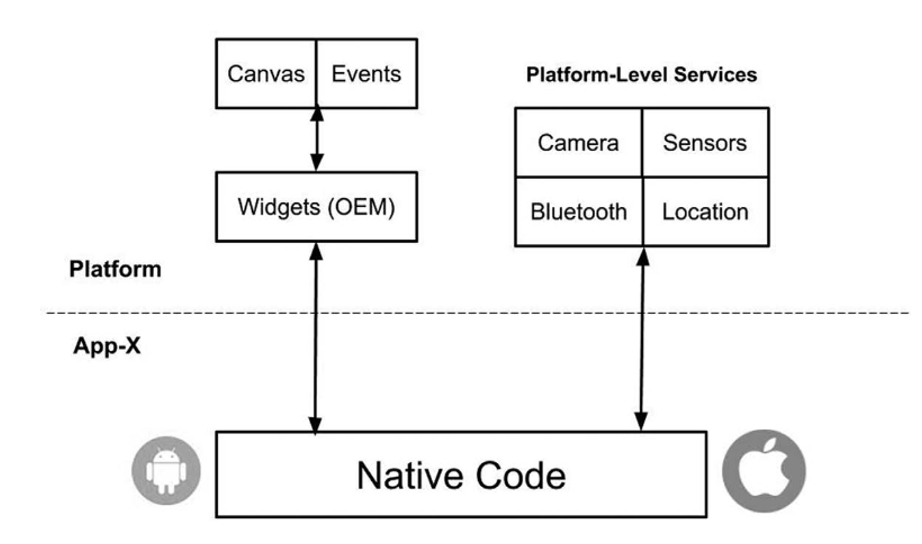
\includegraphics[width=15cm,height=8cm]{Images/system/flutter_native_code.png}
  \caption[Kiến trúc ứng dụng của hệ thống gốc]{\bfseries \fontsize{12pt}{0pt}
  \selectfont Kiến trúc ứng dụng của hệ thống gốc}
  \label{flutter_native_code} %đặt tên cho ảnh
\end{figure}

Hình ảnh trên thể hiện sự tương tác giữa Native Code và các dịch vụ của Platform một cách trực tiếp, nói cách khác, sử dụng
native code chúng ta có thể truy cập đến mọi services một cách nhanh chóng và thuận tiện nhất. Tuy nhiên việc thực hiện
code trên native cũng tương đối khó và đòi hỏi kinh nghiệm vì cấu trúc phức tạp và có hiểu biết về hệ điều hành.

\begin{figure}[H]
  \centering
  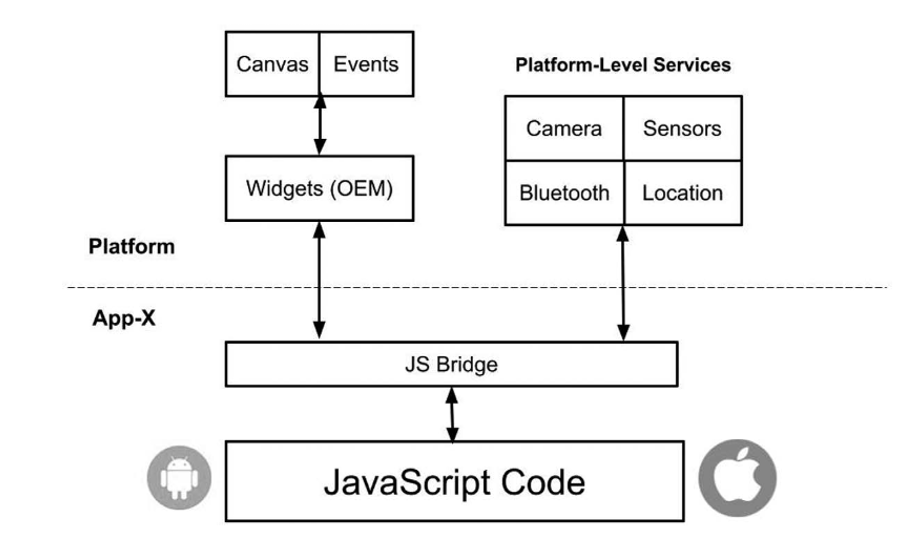
\includegraphics[width=15cm,height=8cm]{Images/system/flutter_JS.png}
  \caption[Kiến trúc ứng dụng của hệ thống sử dụng cầu nối Javascript]{\bfseries \fontsize{12pt}{0pt}
  \selectfont Kiến trúc ứng dụng của hệ thống sử dụng cầu nối Javascript}
  \label{flutter_JS} %đặt tên cho ảnh
\end{figure}

Tiếp theo, để xử lý những vấn đề gặp phải ở trên, giải pháp ở đây đó chính là sử dụng một cầu nối, cầu nối Javascript (một ngôn ngữ lập trình bậc cao)
sẽ giảm tải việc không phải chạm đến native code, đơn giản hoá việc code ứng dụng, nhược điểm là tốc độ xử lý và chạy ứng
dụng sẽ chậm hơn vì phải chuyển từ Javascript qua Native Code khi chạy. 

\begin{figure}[H]
  \centering
  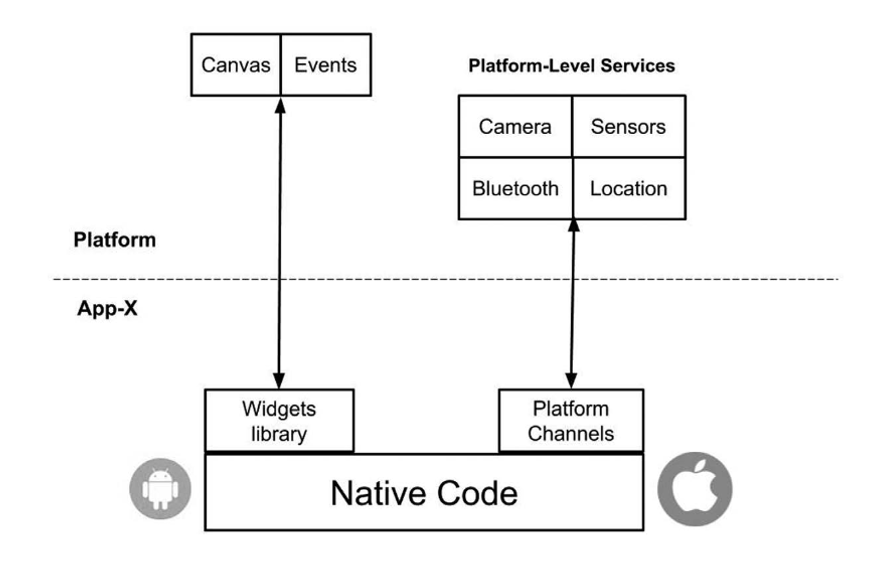
\includegraphics[width=15cm,height=8cm]{Images/system/flutter_dart.png}
  \caption[Kiến trúc ứng dụng của hệ thống sử dụng Method Channel Flutter]{\bfseries \fontsize{12pt}{0pt}
  \selectfont Kiến trúc ứng dụng của hệ thống sử dụng Method Channel Flutter}
  \label{flutter_dart} %đặt tên cho ảnh
\end{figure}

Giải pháp của Flutter là việc xây dựng sẵn Widget tương tác trực tiếp với Native Code, người dùng chỉ cần gọi Widget và tuỳ
biến dựa trên mong muốn, và Method Channel cho việc phát triển những chức năng mà Flutter chưa thực sự hỗ trợ. Việc kết hợp này
giúp cho tốc độ xử lý nhanh và đảm bảo có chiều sâu khi hỗ trợ cả Native Code bắt kỳ khi nào chúng ta cần.


\paragraph{Firebase}
\mbox{}

Ứng dụng di động của bệnh nhân và bác sĩ sử dụng Firebase Firestore để lưu trữ tin nhắn và trong tương lai sẽ sử dụng Firebase
Messaging để gửi thông báo đến cho người nhận. Dưới đây là phần giới thiệu của chúng em về Firebase Firestore:

Firebase Firestore: là một cơ sở dữ liệu NoSQL của Firebase, cho phép bạn lưu trữ và đồng bộ dữ liệu trong thời gian thực giữa ứng dụng của bạn và cơ sở dữ liệu trên đám mây. Firestore được thiết kế để cung cấp hiệu suất cao, đáng tin cậy và dễ sử dụng cho việc lưu trữ và truy vấn dữ liệu.
Đặc điểm của Firebase Firestore bao gồm:
\begin{itemize} 
  \item Lưu trữ dữ liệu dưới dạng tài liệu (document) và bộ sưu tập (collection) có cấu trúc linh hoạt
  \item Hỗ trợ lắng nghe sự thay đổi dữ liệu trong thời gian thực thông qua tính năng "realtime updates"
  \item Được tích hợp sâu với các sản phẩm và dịch vụ khác của Firebase, như Firebase Authentication, Firebase Cloud Functions, và Firebase Cloud Messaging
  \item Có SDK hỗ trợ nhiều nền tảng, bao gồm Android, iOS, web và cả Flutter.
\end{itemize}

% //TODO: add image

\paragraph{Bluetooth Low Energy}
\mbox{}

Ứng dụng di động của bệnh nhân sử dụng Bluetooth với công nghệ Bluetooth Low Energy để truyền/nhận dữ liệu giữa ứng dụng di
động với thiết bị IOT. BLE được thiết kế để tiết kiệm năng lượng và thích hợp cho các ứng dụng yêu cầu tiêu thụ điện năng thấp 
và phạm vi hoạt động ngắn, rất phù hợp với thiết bị điện tim cần truyền dữ liệu liên tục đến ứng dụng. Trong ứng dụng di động này, chúng
em sử dụng đến hai khái niệm thường dùng trong BLE đó là Service và Characteristic.


\begin{itemize} 
  \item Service: được định danh bằng UUID, dùng để định nghĩa một chức năng cụ thể của thiết bị
  \item Characteristic: được định danh bằng UUID, thuộc về một service nhất định và có thể thực hiện việc đọc, ghi cũng như lắng nghe
\end{itemize}

Việc thực hiện lắng nghe Characteristic và lấy dữ liệu ra là chìa khoá của Bluetooth trong ứng dụng lần này.
  \begin{figure}[H]
        \centering
        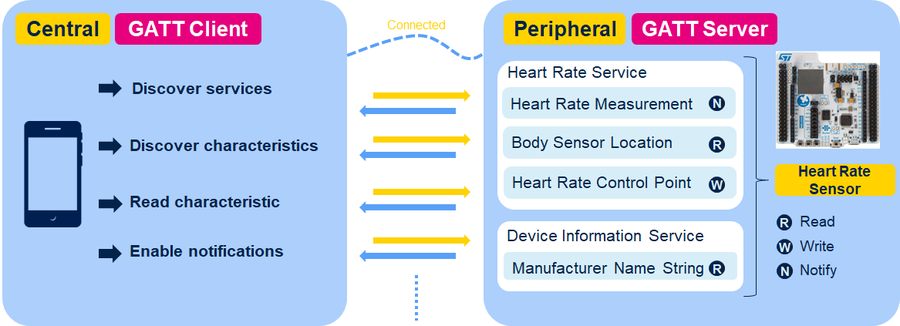
\includegraphics[width=16cm,height=8cm]{Images/system/ble_services.png}
        \caption[Ví dụ mô tả chức năng của Bluetooth Low Energy]{\bfseries \fontsize{12pt}{0pt}
        \selectfont Ví dụ mô tả chức năng của Bluetooth Low Energy}
        \label{ble_services} %đặt tên cho ảnh
  \end{figure}

  Hình \ref{ble_services} mô tả cách mà dữ liệu sẽ được truyền/nhận hay lắng nghe thông qua Write/Read/Notify. 
  Với Central (đại diện cho thiết bị di động), Peripheral đại diện cho thiết bị ngoại vi (thiết bị đo), sau khi kết nối giữa chúng 
  được thiết lập, việc giao tiếp giữa chúng phụ thuộc vào việc chúng ta sẽ kết nối với đúng UUID của từng services hay
  characteristic như đã được giới thiệu ở trên.

\subsubsection{Server và Website}

\paragraph{NodeJs}
\mbox{}

Node.js là một nền tảng phát triển ứng dụng mã nguồn mở cực kỳ mạnh mẽ và đa dạng, giúp các nhà phát triển xây dựng các ứng dụng web và dịch vụ server-side với hiệu suất cao và khả năng mở rộng linh hoạt. Được ra đời vào năm 2009, Node.js đã nhanh chóng trở thành một trong những công nghệ phổ biến nhất trong cộng đồng lập trình viên và được ứng dụng rộng rãi trong các dự án phức tạp cũng như các ứng dụng thời gian thực.

Một trong những điểm mạnh nổi bật của Node.js là sự hỗ trợ tốt cho kiến trúc không đồng bộ (asynchronous architecture). Bản chất của kiến trúc này là khả năng xử lý đa luồng (multithreading) không đồng bộ, giúp ứng dụng có thể xử lý nhiều yêu cầu cùng một lúc mà không phải chờ đợi hoàn thành từng yêu cầu trước. Điều này cho phép Node.js xử lý các yêu cầu I/O (Input/Output) nặng như truy vấn cơ sở dữ liệu, đọc/ghi dữ liệu từ tập tin, hay gửi và nhận các yêu cầu HTTP một cách hiệu quả và nhanh chóng. Sự không đồng bộ cũng giúp tăng hiệu suất cho ứng dụng, đồng thời tiết kiệm tài nguyên hệ thống.

Node.js được xây dựng dựa trên JavaScript, ngôn ngữ lập trình phổ biến và có tính linh hoạt cao. Sự hòa quyện giữa Node.js và JavaScript cho phép phát triển viên sử dụng cùng một ngôn ngữ cho cả phía client và phía server, giúp đơn giản hóa việc phát triển và duy trì mã nguồn. Ngoài ra, cộng đồng phát triển JavaScript rất lớn và đầy đủ tài nguyên học tập và hỗ trợ trực tuyến, điều này làm cho việc học và sử dụng Node.js trở nên dễ dàng và thuận tiện.

Vì Node.js là mã nguồn mở, nên nó rất linh hoạt và có khả năng tùy chỉnh cao. Phát triển viên có thể sửa đổi và mở rộng các tính năng của Node.js tùy theo nhu cầu của dự án một cách dễ dàng. Hơn nữa, Node.js có cộng đồng lớn và năng động, luôn cập nhật và cải tiến mã nguồn để đáp ứng yêu cầu của các dự án phức tạp và đa dạng. Cộng đồng Node.js cũng cung cấp rất nhiều các thư viện và module mở rộng, giúp tăng tính năng và hiệu suất của ứng dụng.

Một trong những ưu điểm nổi bật của Node.js là hỗ trợ đa nền tảng (cross-platform), cho phép chạy ứng dụng trên nhiều hệ điều hành khác nhau như Windows, macOS, Linux, và nhiều nền tảng khác. Điều này giúp đơn giản hóa quá trình triển khai và triển khai ứng dụng trên nhiều môi trường mà không cần thay đổi mã nguồn.

Một ưu điểm khác của Node.js là hỗ trợ tốt cho việc xây dựng các ứng dụng thời gian thực (real-time applications). Điều này rất hữu ích trong việc xây dựng các ứng dụng trò chơi trực tuyến, ứng dụng trò chuyện (chat applications), hay ứng dụng giao tiếp thời gian thực. Cơ chế WebSocket được tích hợp sẵn trong Node.js giúp kết nối và truyền thông dữ liệu giữa server và client một cách liên tục và nhanh chóng.

Bên cạnh đó, Node.js cũng hỗ trợ các thư viện và giao thức mạng như HTTP, HTTPS, TCP, và UDP, cho phép phát triển viên xây dựng các ứng dụng mạng phức tạp và mạnh mẽ. Node.js cũng cung cấp khả năng tạo máy chủ đơn giản và hiệu quả, giúp xây dựng các ứng dụng web phức tạp với khả năng mở rộng linh hoạt.

Trong việc lưu trữ dữ liệu, Node.js hỗ trợ cơ chế xử lý dữ liệu không đồng bộ, giúp tối ưu hóa hiệu suất của ứng dụng trong việc truy xuất và lưu trữ dữ liệu vào cơ sở dữ liệu. Node.js cũng hỗ trợ các cơ sở dữ liệu phổ biến như MySQL, PostgreSQL, MongoDB, và Redis, cho phép phát triển viên lựa chọn cơ sở dữ liệu phù hợp với yêu cầu của dự án.

Ngoài ra, Node.js còn hỗ trợ các tiện ích cho việc phát triển ứng dụng như gỡ lỗi (debugging), kiểm thử (testing), và quản lý gói (package management) thông qua npm (Node Package Manager). Việc sử dụng các công cụ và thư viện này giúp đơn giản hóa việc phát triển và nâng cao chất lượng của mã nguồn.

Trong quá trình triển khai ứng dụng, Node.js hỗ trợ dễ dàng tích hợp với các công cụ triển khai (deployment tools) như Docker và Kubernetes, giúp đơn giản hóa quá trình triển khai và vận hành ứng dụng trên các môi trường khác nhau.

Tổng kết lại, Node.js là một nền tảng phát triển ứng dụng đa dạng và mạnh mẽ, với nhiều ưu điểm nổi trội như kiến trúc không đồng bộ, tích hợp với JavaScript, đa nền tảng, hỗ trợ ứng dụng thời gian thực, và cộng đồng lớn hỗ trợ phong phú. Với những lợi ích đáng kể này, Node.js đã trở thành một lựa chọn ưu việt cho việc xây dựng các ứng dụng web và dịch vụ server-side hiệu quả và mạnh mẽ.

\paragraph{Javascript}
\mbox{}

JavaScript là một ngôn ngữ lập trình thông dịch, đa mục đích và được sử dụng phổ biến trên web. Nó ra đời vào năm 1995 bởi Brendan Eich, khi còn là một ngôn ngữ lập trình đơn giản để cung cấp tính năng tương tác và hiệu ứng động cho trang web. Tuy nhiên, từ đó đến nay, JavaScript đã trở thành một trong những ngôn ngữ lập trình quan trọng nhất trên thế giới, vượt qua giới hạn trang web và mở rộng sang nhiều lĩnh vực phát triển phần mềm khác nhau.

Một trong những yếu tố quan trọng đóng góp vào sự phổ biến của JavaScript là việc nó được tích hợp một cách tự nhiên và mạnh mẽ với các trình duyệt web. Trước khi JavaScript xuất hiện, việc tạo ra hiệu ứng động và tương tác trên trang web đòi hỏi sự hỗ trợ của các ngôn ngữ lập trình phía server như PHP hoặc các công nghệ khác. JavaScript đã định hình lại cách các ứng dụng web tương tác và hiển thị nội dung, giúp chúng trở nên đa dạng và mạnh mẽ hơn.

JavaScript là một ngôn ngữ linh hoạt và dễ tiếp cận, cho phép người phát triển xây dựng các ứng dụng phong phú và phức tạp với giao diện tương tác, kiểu dáng đẹp mắt và tính năng đa dạng. Ngôn ngữ này hỗ trợ một loạt các kiểu dữ liệu như số, chuỗi, mảng, đối tượng và hỗ trợ xử lý chuỗi, số học, ngày tháng, và các phép tính logic phức tạp.

Một điểm mạnh của JavaScript là khả năng xử lý các sự kiện (event) và gắn kết chúng vào các thành phần trên trang web. Sự kiện là những hành động như nhấp chuột, nhập liệu từ bàn phím, hoặc thay đổi trạng thái của trang web. JavaScript cho phép người phát triển xử lý các sự kiện này và thay đổi nội dung hoặc hành vi của trang web một cách linh hoạt, đáp ứng tương tác của người dùng.

Ngoài ra, JavaScript còn hỗ trợ các khái niệm cấu trúc dữ liệu và kiểu dữ liệu linh hoạt như đối tượng (object), mảng (array), và chuỗi (string). Điều này cho phép người phát triển xây dựng các ứng dụng phức tạp và có tính mô đun cao, giúp quản lý mã nguồn dễ dàng và giảm thiểu lỗi trong quá trình phát triển.

Một trong những tính năng đáng chú ý của JavaScript là khả năng thực hiện các yêu cầu mạng bất đồng bộ (asynchronous) thông qua việc sử dụng các API như XMLHttpRequest (XHR) hay Fetch API. Điều này cho phép trang web tương tác với các dịch vụ web và cơ sở dữ liệu một cách hiệu quả mà không làm trì hoãn trình duyệt.

JavaScript cũng hỗ trợ việc tạo ra các ứng dụng web động, đặc biệt là những ứng dụng đơn trang (single-page applications - SPA). SPA là mô hình phát triển ứng dụng web mà trang web chỉ tải một lần duy nhất khi người dùng truy cập, và sau đó các tương tác tiếp theo được thực hiện một cách bất đồng bộ thông qua JavaScript để cập nhật nội dung và thay đổi giao diện mà không cần tải lại trang. Điều này giúp tăng tốc độ và trải nghiệm người dùng.

Một yếu tố quan trọng khác là cộng đồng JavaScript rất đông đảo và nhiệt tình. Có rất nhiều người dùng và nhà phát triển trên toàn thế giới đóng góp và chia sẻ mã nguồn, thư viện, framework và các tài liệu học tập trực tuyến. Điều này làm cho việc học và sử dụng JavaScript trở nên dễ dàng và thuận tiện, đồng thời giúp phát triển viên giải quyết các vấn đề và thách thức trong quá trình xây dựng ứng dụng.

Một trong những hướng phát triển quan trọng của JavaScript là sự phát triển của các framework và thư viện mã nguồn mở như React, Angular, và Vue.js. Các framework này giúp người phát triển xây dựng các ứng dụng web phức tạp và mạnh mẽ một cách dễ dàng và hiệu quả hơn, đồng thời đảm bảo tính tương thích và bảo mật.

Tuy nhiên, JavaScript cũng có một số hạn chế như việc thực hiện mã nguồn phức tạp có thể dẫn đến các vấn đề bảo mật và hiệu suất. Để giải quyết vấn đề này, người phát triển cần phải tuân thủ các nguyên tắc phát triển an toàn và tối ưu hóa mã nguồn.

Tổng kết lại, JavaScript là một ngôn ngữ lập trình linh hoạt, mạnh mẽ và phổ biến, có nhiều ưu điểm vượt trội như tích hợp tốt với trình duyệt, đa dạng kiểu dữ liệu, khả năng thực hiện bất đồng bộ, và cộng đồng phát triển mạnh mẽ. JavaScript đã định hình lại cách các ứng dụng web tương tác và được sử dụng rộng rãi trong nhiều lĩnh vực phát triển phần mềm. Sự phát triển của các framework và thư viện JavaScript giúp người phát triển xây dựng các ứng dụng web phức tạp và mạnh mẽ một cách dễ dàng và hiệu quả hơn.

\paragraph{AdminJS}
\mbox{}

AdminJS là một framework mã nguồn mở được thiết kế để hỗ trợ phát triển các trang quản lý (admin dashboard) dễ dàng và nhanh chóng. Với AdminJS, người phát triển có thể xây dựng các giao diện quản lý phức tạp và mạnh mẽ một cách dễ dàng và hiệu quả, giúp quản lý và điều hành hệ thống, ứng dụng hoặc dịch vụ một cách thuận tiện và hiệu quả hơn.

Một trong những ưu điểm nổi bật của AdminJS là tích hợp các tính năng và chức năng phong phú sẵn có, giúp giảm thiểu thời gian và công sức trong việc xây dựng giao diện quản lý. AdminJS cung cấp các thành phần giao diện (UI components) sẵn có cho việc quản lý các bảng dữ liệu (data tables), hiển thị các biểu đồ thống kê, tạo các biểu mẫu nhập liệu (form fields) và nhiều tính năng khác. Nhờ vậy, người phát triển không cần phải viết mã nguồn từ đầu mà vẫn có thể xây dựng các trang quản lý đẹp mắt và chuyên nghiệp.

AdminJS hỗ trợ tích hợp với nhiều loại cơ sở dữ liệu phổ biến như MongoDB, PostgreSQL, MySQL, và SQLite, giúp tương tác và quản lý dữ liệu một cách dễ dàng. Ngoài ra, nó cũng hỗ trợ tích hợp với các framework và thư viện phổ biến như Express.js, Nest.js, và các thư viện mã nguồn mở khác. Tích hợp với các công nghệ này giúp AdminJS trở nên linh hoạt và dễ dàng tích hợp vào các dự án sẵn có.

Một tính năng quan trọng của AdminJS là khả năng tùy chỉnh và mở rộng. Người phát triển có thể tùy chỉnh các thành phần giao diện sẵn có để phù hợp với yêu cầu và phong cách của dự án. Điều này giúp tạo ra các trang quản lý có giao diện độc đáo và phù hợp với thương hiệu của dự án. Ngoài ra, người phát triển cũng có thể mở rộng và thêm các tính năng tùy chỉnh theo yêu cầu của dự án một cách dễ dàng.

AdminJS cũng hỗ trợ tích hợp các tính năng bảo mật và xác thực. Người phát triển có thể dễ dàng thiết lập và quản lý các quyền truy cập và vai trò người dùng trên các trang quản lý. Điều này giúp bảo mật và bảo vệ dữ liệu quan trọng khỏi việc truy cập trái phép. AdminJS cũng hỗ trợ tích hợp với các công nghệ bảo mật như JSON Web Token (JWT), Passport.js và các cơ chế xác thực khác.

Một điểm mạnh nữa của AdminJS là sự hỗ trợ mạnh mẽ từ cộng đồng. AdminJS có một cộng đồng đông đảo và năng động, luôn cập nhật và đóng góp cho mã nguồn để nâng cao tính năng và hiệu suất của framework. Cộng đồng cũng cung cấp rất nhiều tài liệu học tập và hỗ trợ trực tuyến, giúp người phát triển học hỏi và giải quyết các vấn đề trong quá trình xây dựng giao diện quản lý.

Ngoài ra, AdminJS còn hỗ trợ tích hợp với các công cụ phát triển phổ biến như VSCode, Sublime Text, và Atom, giúp tăng cường trải nghiệm phát triển và giảm thiểu lỗi trong quá trình phát triển. Nó cũng hỗ trợ tích hợp với các công cụ quản lý mã nguồn như Git và GitHub, giúp quản lý và kiểm soát phiên bản mã nguồn một cách hiệu quả.

Tóm lại, AdminJS là một framework mạnh mẽ và linh hoạt để xây dựng các trang quản lý (admin dashboard) dễ dàng và nhanh chóng. Với các tính năng và chức năng phong phú, tích hợp dễ dàng với nhiều loại cơ sở dữ liệu và khả năng tùy chỉnh mạnh mẽ, AdminJS giúp người phát triển xây dựng các giao diện quản lý chuyên nghiệp và mạnh mẽ một cách dễ dàng và hiệu quả. Sự hỗ trợ mạnh mẽ từ cộng đồng và tích hợp với các công cụ phát triển giúp tăng cường trải nghiệm phát triển và đảm bảo chất lượng của mã nguồn.

\paragraph{MySQL}
\mbox{}

MySQL là một hệ quản trị cơ sở dữ liệu mã nguồn mở phổ biến và mạnh mẽ, được sử dụng rộng rãi trong nhiều ứng dụng và dự án phát triển phần mềm. MySQL ra đời vào năm 1995, do công ty TcX phát triển và sau đó được mua lại bởi công ty MySQL AB. Hiện nay, MySQL thuộc sở hữu của Oracle Corporation sau khi Oracle mua lại Sun Microsystems - công ty mẹ của MySQL AB vào năm 2010.

MySQL là hệ quản trị cơ sở dữ liệu (DBMS - Database Management System) dựa trên mô hình quan hệ (relational database) và sử dụng ngôn ngữ truy vấn cấu trúc (Structured Query Language - SQL) để thực hiện các thao tác truy vấn dữ liệu. Mô hình quan hệ của MySQL cho phép lưu trữ và quản lý dữ liệu trong các bảng có mối quan hệ với nhau, tạo điều kiện để thực hiện các truy vấn phức tạp và hiệu quả.

MySQL hỗ trợ nhiều loại dữ liệu phổ biến như số, chuỗi, ngày tháng, boolean, và các kiểu dữ liệu đặc biệt khác như JSON và các kiểu dữ liệu không gian (spatial data types). Điều này giúp người dùng lưu trữ và xử lý các loại dữ liệu khác nhau một cách linh hoạt và hiệu quả.

Một trong những ưu điểm quan trọng của MySQL là hiệu suất cao và khả năng mở rộng linh hoạt. MySQL được tối ưu hóa để xử lý các yêu cầu truy vấn nhanh chóng và hiệu quả, cho phép xử lý hàng triệu hoặc thậm chí hàng tỷ bản ghi một cách mượt mà. Ngoài ra, MySQL cũng hỗ trợ tính năng phân chia dữ liệu (sharding) và nhân bản dữ liệu (replication), giúp tăng khả năng chịu tải và đảm bảo tính sẵn sàng và tin cậy của hệ thống.

MySQL cung cấp các tính năng bảo mật và quản lý người dùng mạnh mẽ. Người quản trị có thể xác định và quản lý các quyền truy cập của người dùng và vai trò của họ trên các bảng và cơ sở dữ liệu. Điều này giúp bảo vệ dữ liệu quan trọng và ngăn chặn truy cập trái phép.

MySQL hỗ trợ các công cụ và giao thức mạng như JDBC, ODBC, và các API kết nối khác, cho phép ứng dụng kết nối và tương tác với cơ sở dữ liệu MySQL từ các ứng dụng phần mềm và trang web khác nhau. MySQL cũng hỗ trợ giao thức kết nối và truy vấn an toàn, giúp đảm bảo tính bảo mật và chống lại các cuộc tấn công từ xa.

MySQL có sự hỗ trợ mạnh mẽ từ cộng đồng và cung cấp rất nhiều tài liệu học tập và hỗ trợ trực tuyến. Cộng đồng MySQL rất đông đảo và năng động, luôn cập nhật và đóng góp cho mã nguồn để nâng cao tính năng và hiệu suất của hệ quản trị cơ sở dữ liệu này.

MySQL cũng hỗ trợ tích hợp với các công cụ phát triển và quản lý mã nguồn như MySQL Workbench, phpMyAdmin và các công cụ khác, giúp quản lý và xem xét dữ liệu một cách thuận tiện và hiệu quả.

Một điểm đáng chú ý nữa của MySQL là tính tương thích với nhiều hệ điều hành và nền tảng khác nhau. MySQL có phiên bản dành cho Windows, macOS và các hệ điều hành Linux khác nhau, giúp người dùng lựa chọn và triển khai phù hợp với môi trường họ sử dụng.

Tóm lại, MySQL là một hệ quản trị cơ sở dữ liệu mã nguồn mở mạnh mẽ và phổ biến, được sử dụng rộng rãi trong nhiều ứng dụng và dự án phát triển phần mềm. Với tính năng hiệu suất cao, khả năng mở rộng linh hoạt, tính bảo mật và quản lý người dùng, sự hỗ trợ từ cộng đồng và tích hợp với nhiều công cụ phát triển, MySQL đã trở thành một lựa chọn ưu việt cho việc quản lý và xử lý cơ sở dữ liệu.


\paragraph{Postman}
\mbox{}

Postman là một ứng dụng máy tính được sử dụng phổ biến trong quá trình phát triển và kiểm thử các dịch vụ web (web service) và các API (Application Programming Interface). Được phát triển bởi công ty Postman Inc., ứng dụng này cung cấp một giao diện đơn giản và dễ sử dụng để gửi các yêu cầu HTTP (HTTP request) và nhận các phản hồi (response) từ các API. Postman giúp người phát triển dễ dàng thử nghiệm và kiểm tra tính năng, hiệu năng và bảo mật của các dịch vụ web và API, từ đó đảm bảo chất lượng và độ tin cậy của ứng dụng.

Một trong những ưu điểm nổi bật của Postman là khả năng gửi các yêu cầu HTTP một cách linh hoạt và dễ dàng. Người dùng có thể tùy chỉnh các yêu cầu HTTP bằng cách thêm các thông số và tham số, cũng như xác định các phương thức HTTP như GET, POST, PUT, DELETE, và nhiều phương thức khác. Điều này giúp người phát triển kiểm tra các chức năng khác nhau của API và dịch vụ web một cách hiệu quả.

Postman cũng hỗ trợ quản lý các môi trường (environments) khác nhau, cho phép người dùng cấu hình các giá trị môi trường như URL, token xác thực, hay các giá trị động khác. Nhờ vậy, người dùng có thể thử nghiệm các yêu cầu API trên nhiều môi trường khác nhau một cách dễ dàng, từ đó giả lập các trường hợp sử dụng và kiểm tra tính ổn định của API.

Một tính năng mạnh mẽ khác của Postman là khả năng tự động hóa các bước kiểm thử và thực hiện các bộ kiểm thử (test suite). Người dùng có thể viết các mã kiểm thử (test script) bằng ngôn ngữ JavaScript để kiểm tra phản hồi từ API và đánh giá tính đúng đắn của dữ liệu trả về. Điều này giúp tăng cường tính tin cậy của các bài kiểm thử và giảm thiểu nguy cơ sai sót từ phía người dùng.

Postman hỗ trợ tích hợp với các công cụ và dịch vụ phổ biến khác như GitHub, Jenkins, và các công cụ kiểm thử liên quan khác. Điều này giúp người phát triển tích hợp Postman vào quy trình phát triển phần mềm tự động một cách dễ dàng, từ việc kiểm tra mã nguồn đến việc chạy các bài kiểm thử tự động.

Postman cung cấp giao diện người dùng thân thiện và trực quan, giúp người dùng dễ dàng thao tác và nắm bắt các tính năng của ứng dụng. Nó cũng hỗ trợ nhiều loại dữ liệu và định dạng như JSON, XML, và form data, giúp người dùng kiểm thử các yêu cầu API đa dạng và phong phú.

Ngoài ra, Postman còn hỗ trợ tích hợp với Postman Cloud, một dịch vụ lưu trữ dữ liệu trực tuyến cho phép người dùng chia sẻ và quản lý các bài kiểm thử và dữ liệu API trực tuyến. Điều này giúp tăng cường sự cộng tác và quản lý dự án trong quá trình phát triển.

Postman đã trở thành một công cụ quan trọng và không thể thiếu trong quá trình phát triển và kiểm thử các ứng dụng và dịch vụ web. Sự dễ dàng sử dụng, tích hợp và tự động hóa giúp tăng cường năng suất và chất lượng của quá trình phát triển, đồng thời giảm thiểu nguy cơ lỗi và tối ưu hóa hiệu suất của ứng dụng.

\subsection{Triển khai ứng dụng}
Trong quá trình triển khai ứng dụng, chúng em sử dụng dịch vụ Elastic Compute
 Cloud (EC2) của AWS để chạy ứng dụng và sử dụng dịch vụ Relational Database Service
  (RDS) để lưu trữ cơ sở dữ liệu của ứng dụng. Việc sử dụng EC2 và RDS giúp
   chúng em tối ưu hóa việc quản lý hệ thống, đảm bảo tính sẵn sàng và
    mở rộng khả năng chịu tải cho ứng dụng.

\subsubsection{Triển khai ứng dụng Web trên AWS EC2}
\begin{itemize}
  \item Tạo máy ảo EC2: Chúng em đã tạo một EC2 instance với loại instance t2.micro. Đây là loại instance nhỏ, phù hợp với các ứng dụng có lưu lượng truy cập thấp hoặc giai đoạn phát triển. Instance này sử dụng kiến trúc 64-bit, cho phép chạy các ứng dụng trên cả hệ thống 32-bit và 64-bit. Bộ nhớ của instance là 1 GiB, đủ để chạy ứng dụng Node.js cùng với các dependencies. Dung lượng lưu trữ 8GB, chúng em đã cài đặt hệ điều hành Linux/UNIX để chạy mã nguồn của ứng dụng.
  

  \begin{figure}[H]
    \centering
    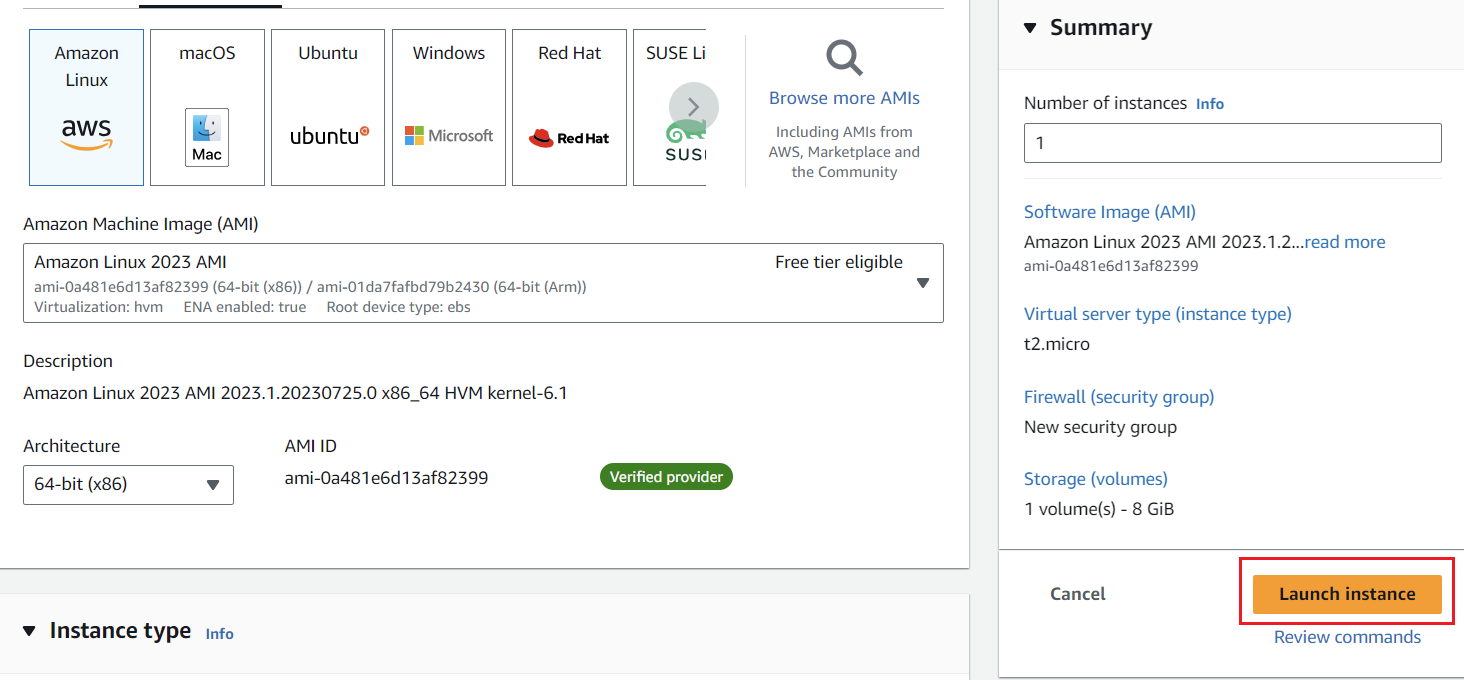
\includegraphics[scale=0.5]{Images/server/deploy/create_ec2.PNG}
    \caption[Tạo máy ảo EC2]{\bfseries \fontsize{12pt}{0pt}
    \selectfont Tạo máy ảo EC2}
    \label{create_ec2} %đặt tên cho ảnh
  \end{figure}

  Sau khi tạo thành công, trên trang dashboad quản lý EC2 sẽ xuất hiện máy ảo mà ta đã tạo vừa xong

  \begin{figure}[H]
    \centering
    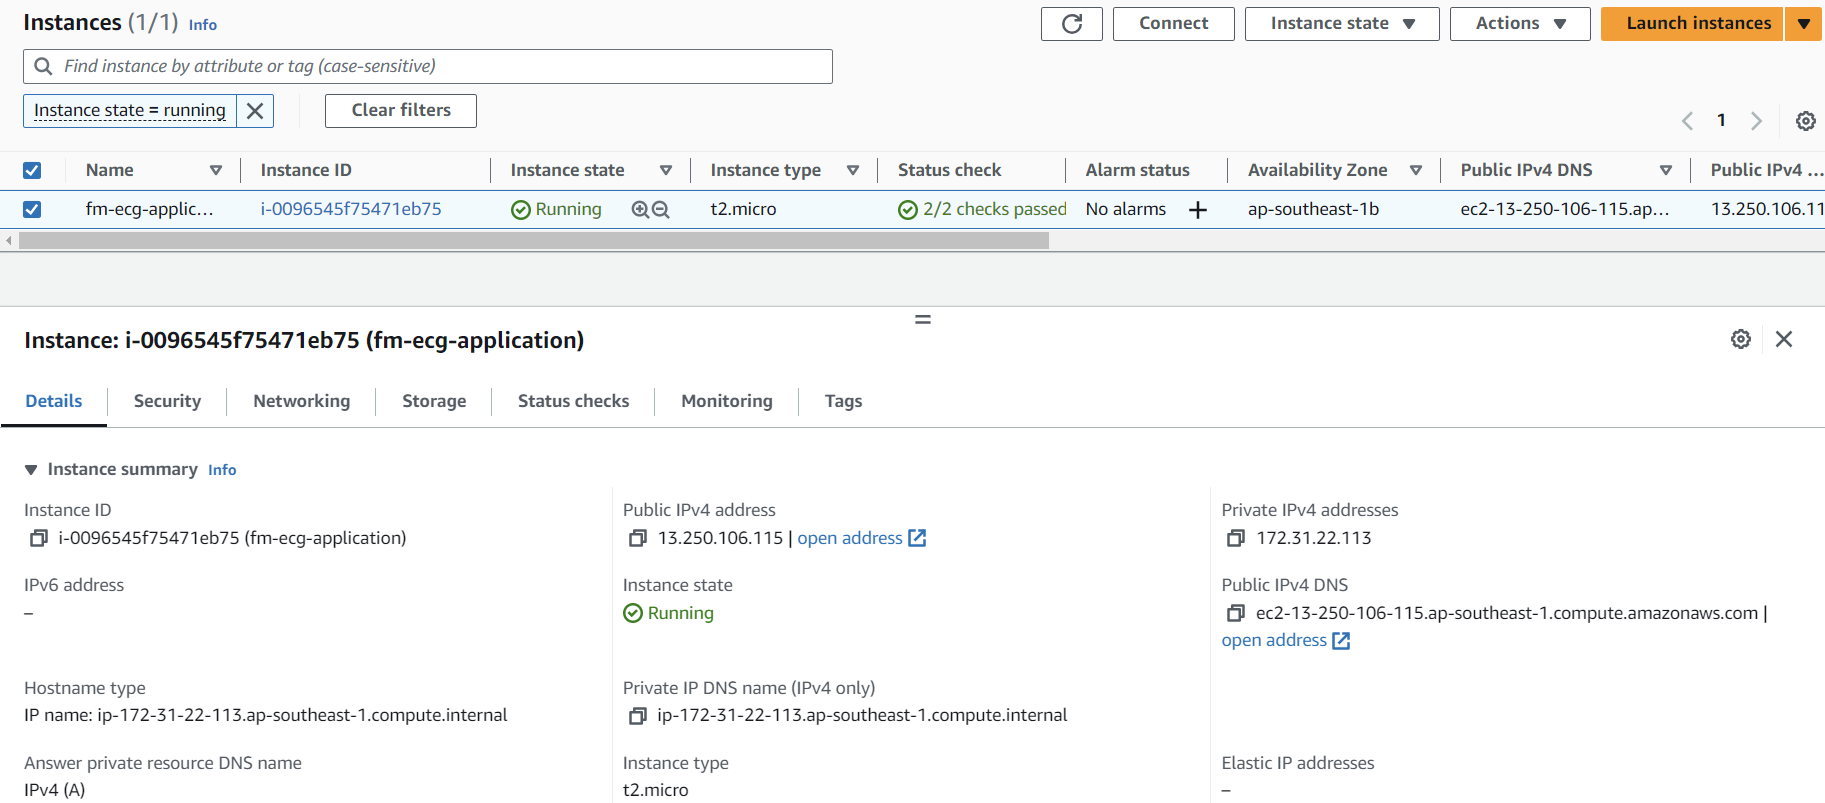
\includegraphics[scale=0.4]{Images/server/deploy/ec2_dashboard.PNG}
    \caption[Trang dashboad quản lý EC2 instance]{\bfseries \fontsize{12pt}{0pt}
    \selectfont Trang dashboad quản lý EC2 instance}
    \label{ec2_dashboard} %đặt tên cho ảnh
  \end{figure}

  Từ trang dashboard, ta sẽ thực hiện kết nối với máy ảo thông qua nút Connect

  \begin{figure}[H]
  \centering
  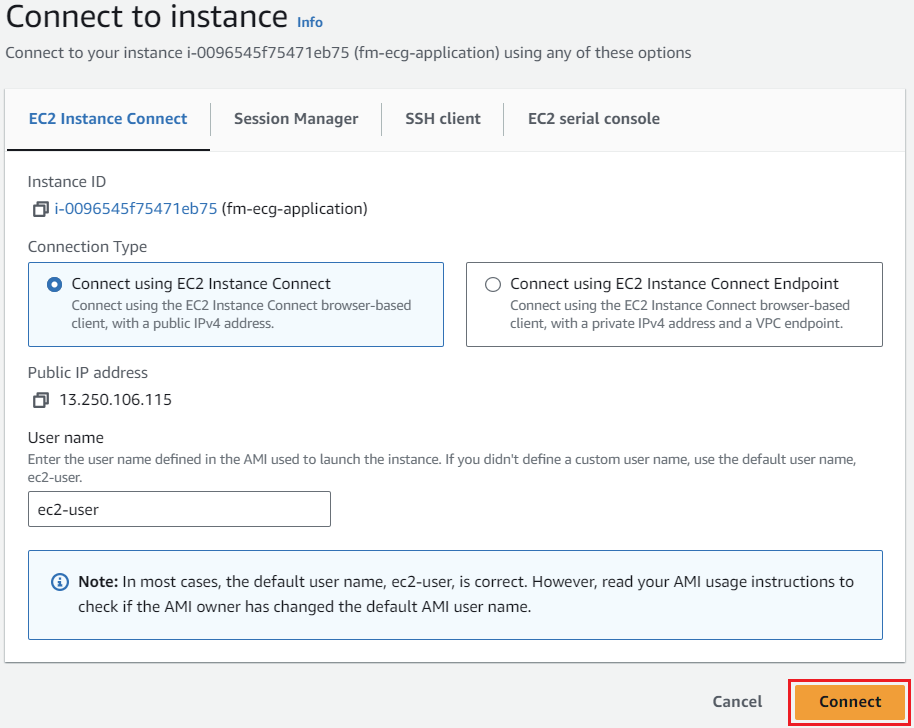
\includegraphics[scale=0.5]{Images/server/deploy/connect_ec2.PNG}
  \caption[Trang kết nối tới máy ảo]{\bfseries \fontsize{12pt}{0pt}
  \selectfont Trang kết nối tới máy ảo}
  \label{connect_ec2} %đặt tên cho ảnh
\end{figure}


  Sau khi kết nối thành công trang console của máy ảo sẽ xuất hiện, từ đây ta có thể thực hiện các thao tác mong muốn trên server thông qua console

  \begin{figure}[H]
    \centering
    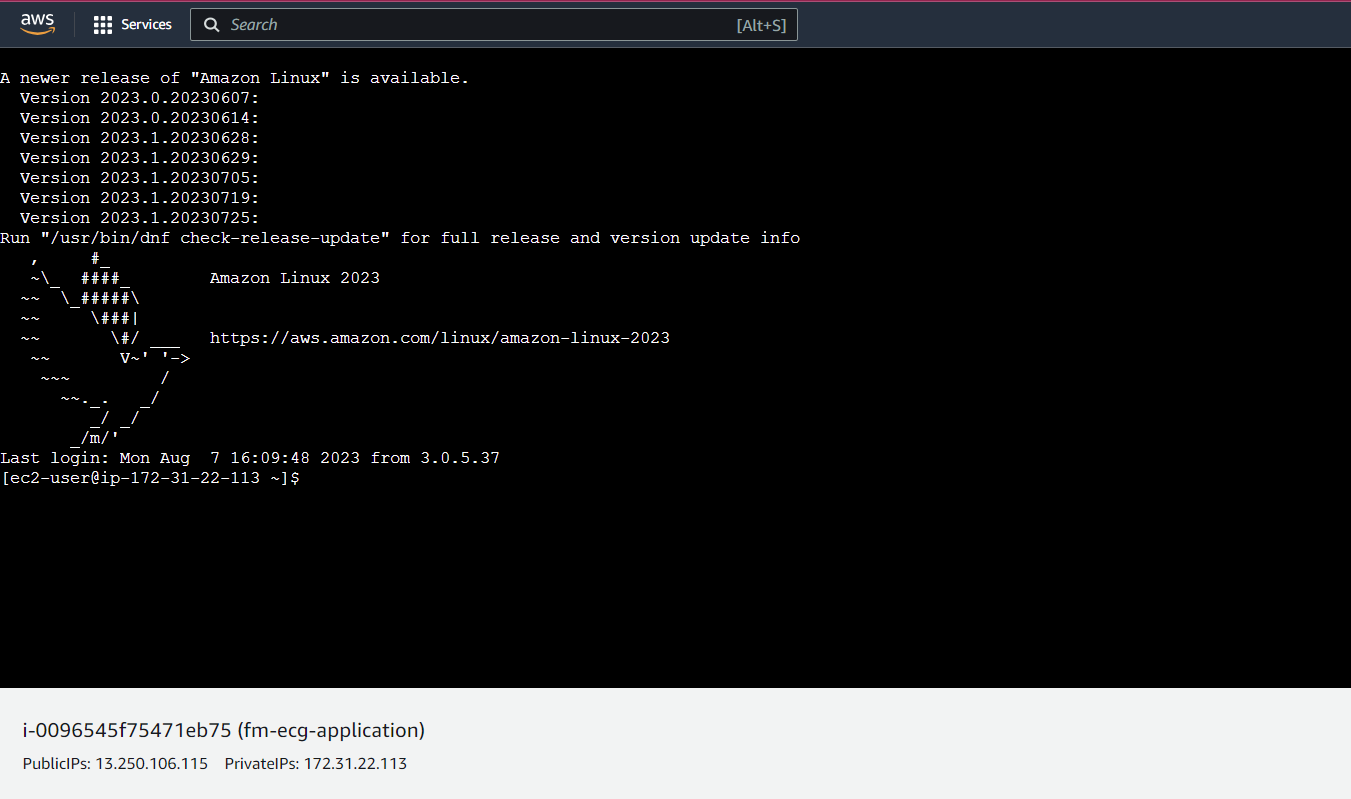
\includegraphics[scale=0.55]{Images/server/deploy/ec2_console.PNG}
    \caption[Trang console của máy ảo]{\bfseries \fontsize{12pt}{0pt}
    \selectfont Trang console của máy ảo}
    \label{ec2_console} %đặt tên cho ảnh
  \end{figure}



  \item Cài đặt các phần mềm và dependencies: Sau khi triển khai máy ảo EC2, chúng em đã cài đặt các phần mềm và dependencies cần thiết để chạy ứng dụng, bao gồm Node.js và các thư viện hỗ trợ và các gói npm cần thiết.
  


  \begin{figure}[H]
    \centering
    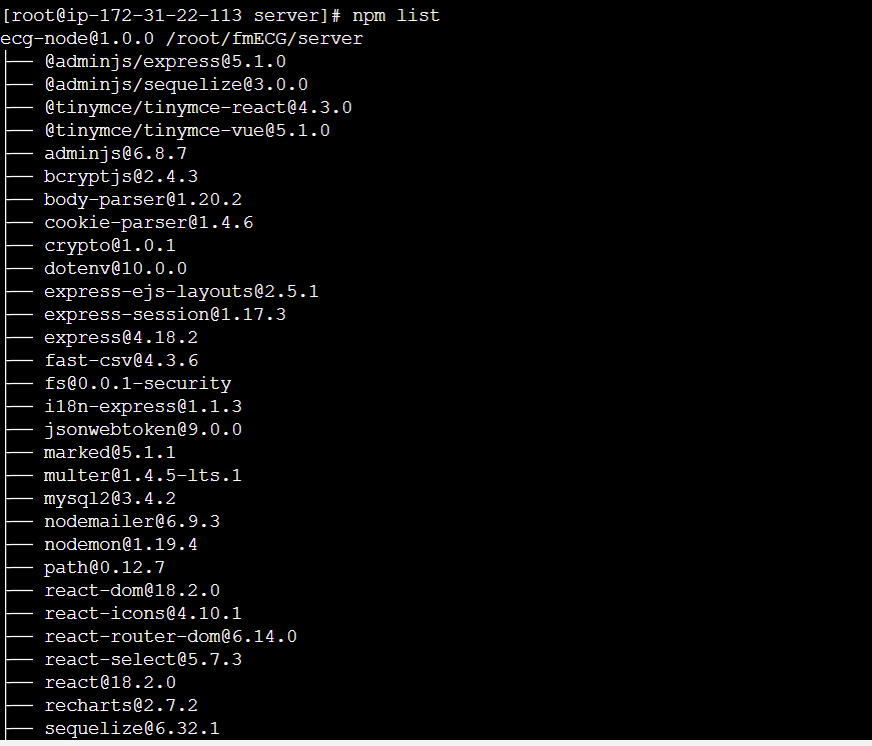
\includegraphics[scale=0.7]{Images/server/deploy/list_node_package.PNG}
    \caption[Các packages và dependencies cần thiết]{\bfseries \fontsize{12pt}{0pt}
    \selectfont Các packages và dependencies cần thiết}
    \label{ec2_dashboard} %đặt tên cho ảnh
  \end{figure}


  \item Tạo và cấu hình môi trường ứng dụng: Chúng em đã tạo môi trường ứng dụng, bao gồm việc cấu hình các biến môi trường, thiết lập các file cấu hình, và chạy các lệnh khởi tạo ban đầu cho ứng dụng.
  \item Triển khai ứng dụng: Tiếp theo, chúng em tải lên mã nguồn của ứng dụng lên máy ảo EC2 thông qua git
  
  \begin{figure}[H]
    \centering
    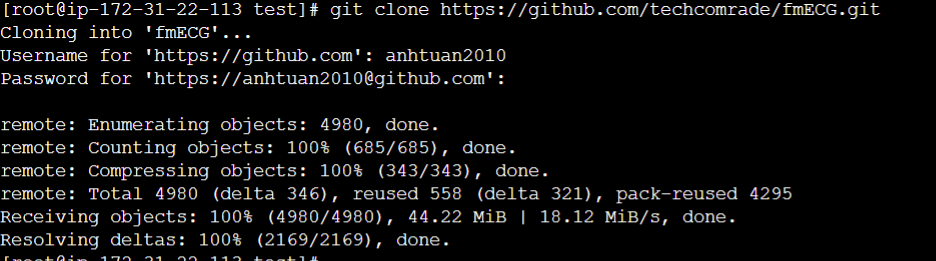
\includegraphics[scale=0.7]{Images/server/deploy/git_ec2.PNG}
    \caption[Tải mã nguồn lên server thông qua git]{\bfseries \fontsize{12pt}{0pt}
    \selectfont Tải mã nguồn lên server thông qua git}
    \label{ec2_dashboard} %đặt tên cho ảnh
  \end{figure}

  \item Mở cổng cho ứng dụng: Chúng em đã mở cổng mạng trên máy ảo EC2 để cho phép ứng dụng lắng nghe các yêu cầu từ internet.
  \item Khởi động ứng dụng: Để khởi động ứng dụng, chúng em chạy các lệnh quản lý quá trình như npm start
  

  \begin{figure}[H]
    \centering
    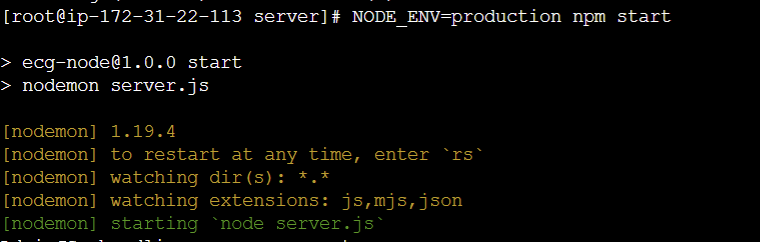
\includegraphics[scale=0.7]{Images/server/deploy/execute_sever.PNG}
    \caption[Chạy ứng dụng]{\bfseries \fontsize{12pt}{0pt}
    \selectfont Chạy ứng dụng}
    \label{execute_sever} %đặt tên cho ảnh
  \end{figure}


\end{itemize}

\subsubsection{Triển khai cơ sở dữ liệu trên RDS}
\begin{itemize}
  \item Tạo cơ sở dữ liệu RDS: Chúng em đã triển khai một cơ sở dữ liệu MySQL trên dịch vụ RDS của AWS. Cơ sở dữ liệu này được đặt tên là "fm\_ecg" và có mật khẩu "fmecgdatabase" để bảo mật. Địa chỉ host của cơ sở dữ liệu là "fm-ecg-database.cx3akkmg3hid.ap-southeast-1.rds.amazonaws.com" cho phép EC2 instance kết nối và truy vấn dữ liệu từ cơ sở dữ liệu. Để truy cập và quản lý cơ sở dữ liệu, chúng em sử dụng tài khoản "admin" với các quyền tương ứng.
  
  \begin{figure}[H]
    \centering
    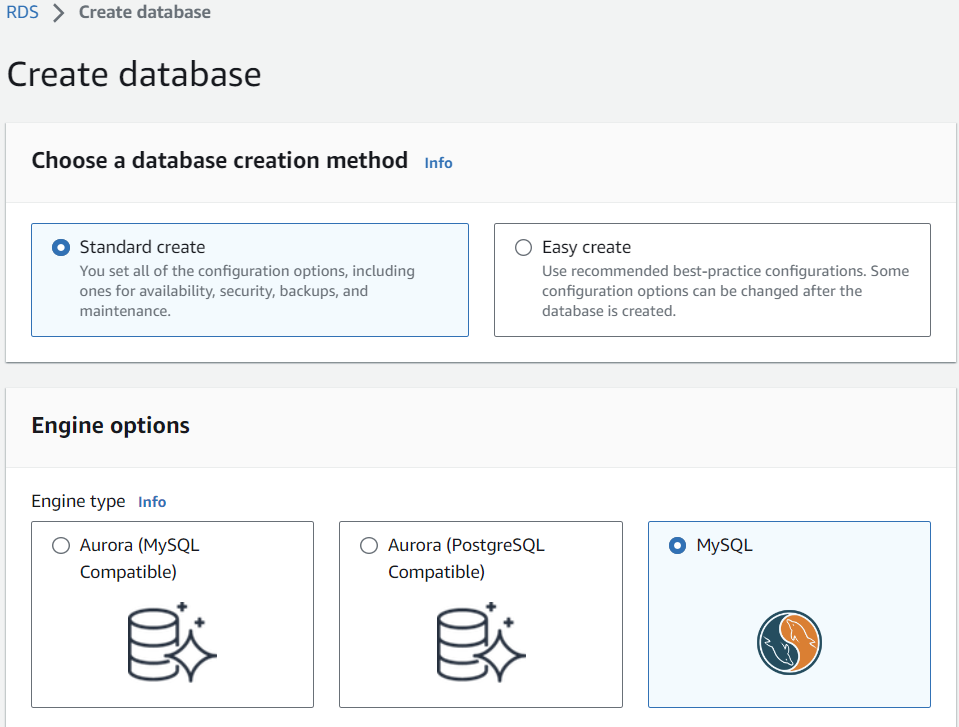
\includegraphics[scale=0.7]{Images/server/deploy/create_rds.PNG}
    \caption[Tạo cơ sở dữ liệu RDS]{\bfseries \fontsize{12pt}{0pt}
    \selectfont Tạo cơ sở dữ liệu RDS}
    \label{create_rds} %đặt tên cho ảnh
  \end{figure}


  \begin{figure}[H]
    \centering
    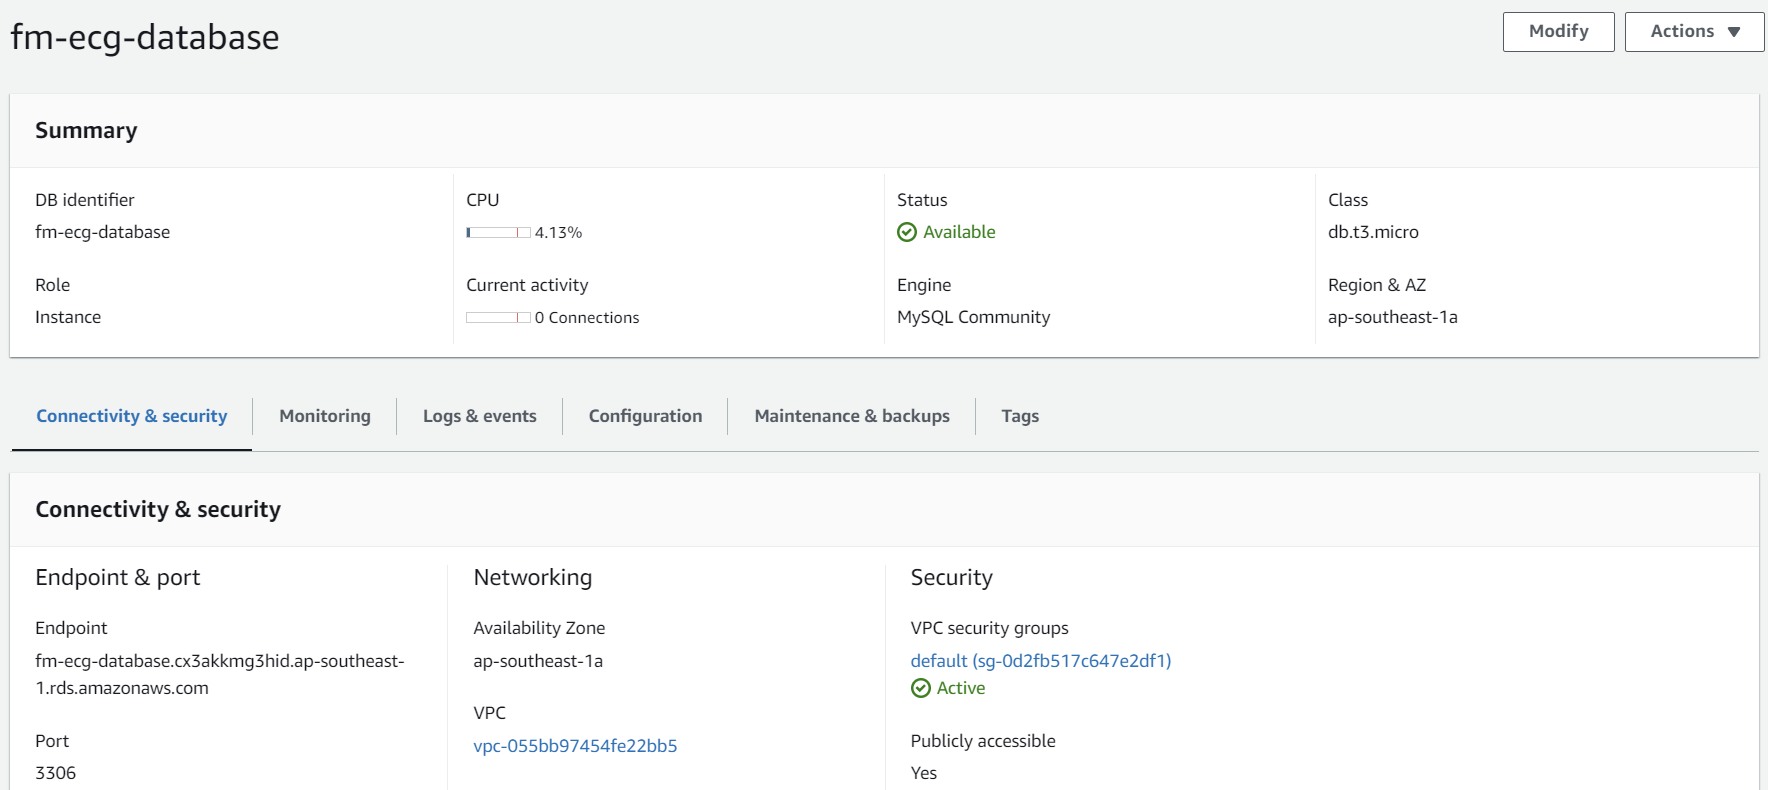
\includegraphics[scale=0.43]{Images/server/deploy/rds_detail.PNG}
    \caption[Cơ sở dữ liệu RDS sau khi tạo thành công]{\bfseries \fontsize{12pt}{0pt}
    \selectfont Cơ sở dữ liệu RDS sau khi tạo thành công}
    \label{rds_detail} %đặt tên cho ảnh
  \end{figure}

  \item Kết nối giữa EC2 và RDS: Chúng em đã cấu hình ứng dụng Node.js chạy trên EC2 instance để kết nối đến cơ sở dữ liệu RDS thông qua thông tin host, tên người dùng và mật khẩu đã cung cấp. Khi ứng dụng gửi các truy vấn SQL đến cơ sở dữ liệu, RDS sẽ xử lý các truy vấn này và trả về kết quả cho ứng dụng.
  

  \begin{figure}[H]
    \centering
    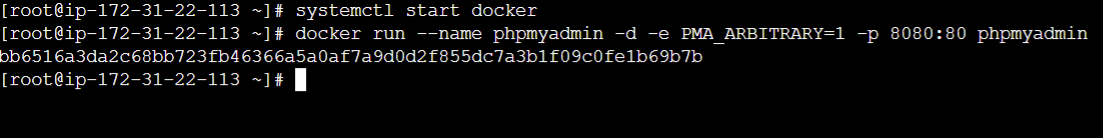
\includegraphics[scale=0.7]{Images/server/deploy/connect_rds_1.PNG}
    \caption[Kết nối giữa EC2 và RDS trên máy ảo EC2]{\bfseries \fontsize{12pt}{0pt}
    \selectfont Kết nối giữa EC2 và RDS trên máy ảo EC2}
    \label{rds_detail} %đặt tên cho ảnh
  \end{figure}

  Sau khi kết nối thành công, ta vào đường dẫn \underline{http://13.250.106.115:8080/} để đăng nhập vào trang quản lý database của hệ thống với tên máy chủ, tài khoản, mật khẩu đã tạo trước đó


  \begin{figure}[H]
    \centering
    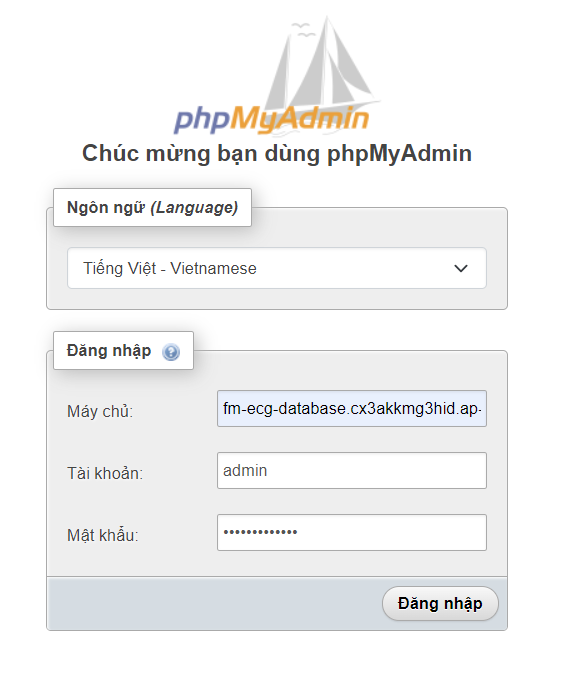
\includegraphics[scale=0.7]{Images/server/deploy/connect_rds_2.PNG}
    \caption[Cơ sở dữ liệu RDS sau khi tạo thành công]{\bfseries \fontsize{12pt}{0pt}
    \selectfont Cơ sở dữ liệu RDS sau khi tạo thành công}
    \label{rds_detail} %đặt tên cho ảnh
  \end{figure}


  \item Backup và giám sát cơ sở dữ liệu: Chúng em đã thiết lập các chính sách sao lưu định kỳ cho cơ sở dữ liệu RDS để đảm bảo an toàn cho dữ liệu và khả năng khôi phục trong trường hợp xảy ra sự cố.
\end{itemize}

\subsubsection{Triển khai ứng dụng di động trên nền tảng Android}
Trong quá trình phát triển ứng dụng di động chúng em có sử dụng máy ảo Android (phiên bản Android API 33) và máy thật
(Android 11 - 13), đồng thời xuất file APK để có thể linh động hơn trong việc triển khai và kiểm thử.

Việc triển khai ứng dụng di động được tự động hoá khi được áp dụng CI/CD (Continous Integration/Continous Development), mỗi khi có
code mới được đẩy lên Github (dịch vụ lưu trữ mã nguồn), sẽ có Github Actions tự động chạy các lệnh để kiểm tra lỗi, cài đặt
các thư viện cần thiết và tạo ra một phiên bản apk cho người dùng tải về và cài đặt. Điều này giúp cho việc phát triển sản phẩm, 
làm việc nhóm trở nên hiệu quả và nhanh chóng hơn.
% //TODO: thêm ref cho CI/CD
% //TODO: thêm ảnh ci/cd, demo một số hình ảnh

\subsection{Kiểm thử}

\subsubsection{Kiểm thử hoạt động của các API}


Môi trường: 

\begin{adjustwidth}{2em}{}
\begin{itemize}
  \item Base URL: http://13.250.106.115/
\end{itemize}
\end{adjustwidth}

Công cụ: Postman - Để xây dựng và thực hiện các yêu cầu API.



\paragraph{API liên quan đến thông tin người dùng}
\mbox{}

Tham khảo bảng \ref{table_api_user} để xem thông tin của các api liên quan

\begin{enumerate}[a)]
  \item URL: GET api/users/profile 
  
  \begin{table}[H]
    \centering
    \caption{\bfseries \fontsize{12pt}{0pt}\selectfont Bảng API liên quan đến tin tức}
    \begin{tabularx}{\textwidth}{
    | >{\raggedright\arraybackslash}m{1cm}
    | >{\raggedright\arraybackslash}X
    | >{\raggedright\arraybackslash}X
    | >{\raggedright\arraybackslash}X
    | >{\raggedright\arraybackslash}m{1cm}|
    }
    \hline
    \bfseries Test case    &\bfseries Điều kiện   &\bfseries Đầu vào 
    &\bfseries Đầu ra mong muốn &\bfseries Kết quả\\ \hline


    TC-1
    & User đã đăng nhập vào hệ thống thành công
    & JWT Cookie có tồn tại
    & 

    Status code: 200 OK

      Response content:

      \{

    "status": "success",

    "data": Thông tin của user

    \}
    
    & OK

    \\ \hline
  
    TC-2
    & User chưa đăng nhập vào hệ thống
    & JWT Cookie không tồn tại
    & 

    Status code: 500 Internal Server Error

      Response content:

      \{

    "status": "error",

    "msg": "An error occurred while retrieving the user profile"

    \}
    
    & OK

    \\ \hline
  
    \end{tabularx}
    \label{table_api_news}
  \end{table}
  

  \item URL: PUT api/users/profile
  
  \begin{table}[H]
    \centering
    \caption{\bfseries \fontsize{12pt}{0pt}\selectfont Bảng API liên quan đến tin tức}
    \begin{tabularx}{\textwidth}{
    | >{\raggedright\arraybackslash}m{1cm}
    | >{\raggedright\arraybackslash}X
    | >{\raggedright\arraybackslash}X
    | >{\raggedright\arraybackslash}X
    | >{\raggedright\arraybackslash}m{1cm}|
    }
    \hline
    \bfseries Test case    &\bfseries Điều kiện   &\bfseries Đầu vào 
    &\bfseries Đầu ra mong muốn &\bfseries Kết quả\\ \hline


    TC-1
    & User đã đăng nhập vào hệ thống thành công
    & Thông tin user muốn cập nhật

    \{

    "name": họ tên,
    "doB": ngày sinh,
    "phone\_number": số điện thoại

\}

    & 

    Status code: 200 OK

      Response content:

      \{

    "status": "success",

    "data": Thông tin của user sau khi cập nhật lại

    \}
    
    & OK

    \\ \hline
  
    TC-2
    & User chưa đăng nhập vào hệ thống
    & Thông tin user muốn cập nhật

    \{

    "name": họ tên,
    "doB": ngày sinh,
    "phone\_number": số điện thoại

\}
    & 

    Status code: 500 Internal Server Error

      Response content:

      \{

    "status": "error",

    "msg": "An error occurred while retrieving the user profile"

    \}
    
    & OK

    \\ \hline
  
    \end{tabularx}
    \label{table_api_news}
  \end{table}
  


  \item URL: PUT api/users/change-password
  
\break

  \begin{xltabular}{\textwidth}{
    | >{\raggedright\arraybackslash}m{1cm}
    | >{\raggedright\arraybackslash}X
    | >{\raggedright\arraybackslash}X
    | >{\raggedright\arraybackslash}X
    | >{\raggedright\arraybackslash}m{1cm}|
    }
    \caption{\bfseries \fontsize{12pt}{0pt}\selectfont Bảng API liên quan đến tin tức}
    % \label{table_api_news}
    \\
    \hline
    \bfseries Test case    &\bfseries Điều kiện   &\bfseries Đầu vào 
    &\bfseries Đầu ra mong muốn &\bfseries Kết quả\\ \hline
  
  
    TC-1
    & User đã đăng nhập vào hệ thống thành công và mật khẩu hiện tại trùng với req.currentPassword, req.newPassword và req.confirmPassword trùng nhau 
    & Thông tin thay đổi mật khẩu
  
    \{
  
      "currentPassword": "123456",
      "newPassword": "1234567",
      "confirmPassword": "1234567"
  
  \}
  
    & 
  
    Status code: 200 OK
  
      Response content:
  
      \{
  
    "status": "success",
  
    msg: "Password changed successfully"
  
    \}
    
    & OK
  
    \\ \hline
  
    TC-2
    & User chưa đăng nhập vào hệ thống
    & Thông tin thay đổi mật khẩu
  
    \{
  
      "currentPassword": mật khẩu hiện tại,
      "newPassword": mật khẩu mới,
      "confirmPassword": xác nhận lại mật khẩu
  
  \}
    & 
  
    Status code: 500 Internal Server Error
  
      Response content:
  
      \{
  
    "status": "error",
  
    "msg": "An error occurred while retrieving the user profile"
  
    \}
    
    & OK
  
    \\ \hline
  
    TC-3
    & User đã đăng nhập vào hệ thống thành công và mật khẩu hiện tại không
    trùng với
    req.currentPassword 
    & Thông tin thay đổi mật khẩu
  
    \{
  
      "currentPassword": "1234568",
      "newPassword": "1234567",
      "confirmPassword": "1234567"
  
  \}
  
    & 
  
    Status code: 401 Unauthorized
  
      Response content:
  
      \{
  
    "status": "error",
  
    msg: "Current password is incorrect"
  
    \}
    
    & OK
  
    \\ \hline
  
    TC-4
    & User đã đăng nhập vào hệ thống thành công và và mật khẩu hiện tại trùng với req.currentPassword, req.newPassword và req.confirmPassword không trùng nhau 
    & Thông tin thay đổi mật khẩu
  
    \{
  
      "currentPassword": "123456",
      "newPassword": "1234567324",
      "confirmPassword": "127"
  
  \}
  
    & 
  
    Status code: 401 Unauthorized
  
      Response content:
  
      \{
  
    "status": "error",
  
    msg: "New password and confirm password do not match"
  
    \}
    
    & OK
  
    \\ \hline
  
    
  
    \end{xltabular}



  \item URL: GET api/users/{:userId}
  
  
  \begin{xltabular}{\textwidth}{
    | >{\raggedright\arraybackslash}m{1cm}
    | >{\raggedright\arraybackslash}X
    | >{\raggedright\arraybackslash}X
    | >{\raggedright\arraybackslash}X
    | >{\raggedright\arraybackslash}m{1cm}|
    }
    \caption{\bfseries \fontsize{12pt}{0pt}\selectfont Bảng API liên quan đến tin tức}
    % \label{table_api_news}
    \\
    \hline
    \bfseries Test case    &\bfseries Điều kiện   &\bfseries Đầu vào 
    &\bfseries Đầu ra mong muốn &\bfseries Kết quả\\ \hline
  
  
    TC-1
    & User ID có tồn tại trên database
    & User ID
  
    & 
  
    Status code: 200 OK
  
      Response content:
  
      \{
  
    "status": "success",
  
    data: Thông tin user
  
    \}
    
    & OK
  
    \\ \hline
  
    TC-2
    & User ID không tồn tại trên database
    & User ID
  
    & 
  
    Status code: 404 Not Found
  
      Response content:
  
      \{
  
    "status": "error",
  
    "msg": "User not found"
  
    \}
    
    & OK
  
    \\ \hline
    
  
    \end{xltabular}

  
\end{enumerate}


\paragraph{API liên quan đến việc xác thực người dùng}
\mbox{}

Tham khảo bảng \ref{table_api_auth} để xem thông tin của các api liên quan



\begin{enumerate}[a)]
  \item URL: POST api/register
  
  \begin{xltabular}{\textwidth}{
    | >{\raggedright\arraybackslash}m{1cm}
    | >{\raggedright\arraybackslash}X
    | >{\raggedright\arraybackslash}X
    | >{\raggedright\arraybackslash}X
    | >{\raggedright\arraybackslash}m{1cm}|
    }
    \caption{\bfseries \fontsize{12pt}{0pt}\selectfont Bảng API liên quan đến tin tức}
    % \label{table_api_news}
    \\
    \hline
    \bfseries Test case    &\bfseries Điều kiện   &\bfseries Đầu vào 
    &\bfseries Đầu ra mong muốn &\bfseries Kết quả\\ \hline
  
  
    TC-1
    & User chưa có tài khoản trên hệ thống
    & Thông tin đăng ký tài khoản

    \{

    "password": "123456789",
    "confirm\_password": "123456789",
    "name": "Anh Tuan",
    "doB": "20-10-2001",
    "email": "test@gmail.com",
    "phone\_number": "0123344562",
    "role": 0

   \}
  
    & 
  
    Status code: 200 OK
  
      Response content:
  
      \{
  
    "status": "success",
  
    data: Thông tin user sau khi đăng ký thành công
  
    \}
    
    & OK
  
    \\ \hline
  
    TC-2
    & User đã có tài khoản trên hệ thống
    & Thông tin đăng ký tài khoản

    \{

    "password": "123456789",
    "confirm\_password": "123456789",
    "name": "Anh Tuan",
    "doB": "20-10-2001",
    "email": "test@gmail.com",
    "phone\_number": "0123344562",
    "role": 0

   \}
  
    & 
  
    Status code: 400 Bad Request
  
      Response content:
  
      \{
  
    "status": "error",
  
    "msg": "Email is already in use"
  
    \}
    
    & OK
  
    \\ \hline


    TC-3
    & User chưa có tài khoản trên hệ thống, req.password và req.confirm\_password không trùng nhau
    & Thông tin đăng ký tài khoản

    \{

    "password": "123456789",

    "confirm\_password": "123456789",

    "name": "Anh Tuan",

    "doB": "20-10-2001",

    "email": "test@gmail.com",

    "phone\_number": "0123344562",

    "role": 0

   \}
  
    & 
  
    Status code: 400 Bad Request
  
      Response content:
  
      \{
  
    "status": "error",
  
    "msg": "Passwords do not match"
  
    \}
    
    & OK
  
    \\ \hline
    
  
    \end{xltabular}

  


  \item URL: POST api/login
  

  \begin{xltabular}{\textwidth}{
    | >{\raggedright\arraybackslash}m{1cm}
    | >{\raggedright\arraybackslash}X
    | >{\raggedright\arraybackslash}X
    | >{\raggedright\arraybackslash}X
    | >{\raggedright\arraybackslash}m{1cm}|
    }
    \caption{\bfseries \fontsize{12pt}{0pt}\selectfont Bảng API liên quan đến tin tức}
    % \label{table_api_news}
    \\
    \hline
    \bfseries Test case    &\bfseries Điều kiện   &\bfseries Đầu vào 
    &\bfseries Đầu ra mong muốn &\bfseries Kết quả\\ \hline
  
  
    TC-1
    & Thông tin tài khoản và mật khẩu hợp lệ
    & Thông tin đăng nhập

    \{

    "email": email của user,
    "password": mật khẩu của user

   \}
  
    & 
  
    Status code: 200 OK
  
      Response content:
  
      \{
  
    "status": "success",
  
    data: Thông tin user sau khi đăng ký thành công
  
    \}
    
    & OK
  
    \\ \hline
  
    TC-2
    & Thông tin tài khoản và mật khẩu không hợp lệ
    & Thông tin đăng nhập

    \{

    "email": email của user,
    "password": mật khẩu của user

   \}
  
   &
  
    Status code: 401 Unauthorized
  
      Response content:
  
      \{
  
    "status": "error",
  
    "msg": "Invalid email or password"
  
    \}
    
    & OK
  
    \\ \hline

  
    \end{xltabular}



  \item URL: GET api/logout
  

  \begin{xltabular}{\textwidth}{
    | >{\raggedright\arraybackslash}m{1cm}
    | >{\raggedright\arraybackslash}X
    | >{\raggedright\arraybackslash}X
    | >{\raggedright\arraybackslash}X
    | >{\raggedright\arraybackslash}m{1cm}|
    }
    \caption{\bfseries \fontsize{12pt}{0pt}\selectfont Bảng API liên quan đến tin tức}
    % \label{table_api_news}
    \\
    \hline
    \bfseries Test case    &\bfseries Điều kiện   &\bfseries Đầu vào 
    &\bfseries Đầu ra mong muốn &\bfseries Kết quả\\ \hline
  
  
    TC-1
    & User đã đăng nhập vào hệ thống
    & JWT Token tồn tại
  
    & 
  
    Status code: 200 OK
  
      Response content:
  
      \{
  
    "status": "success",
  
    "msg": "Logged out successfully"
  
    \}
    
    & OK
  
    \\ \hline
  
    TC-2
    & User chưa đăng nhập vào hệ thống
    & JWT Token không tồn tại
  
   &
  
    Status code: 401 Unauthorized
  
      Response content:
  
      \{
  
    "status": "error",
  
    "msg": "No token found"
  
    \}
    
    & OK
  
    \\ \hline

  
    \end{xltabular}



  \item URL: POST api/reset-password
  


  \begin{xltabular}{\textwidth}{
    | >{\raggedright\arraybackslash}m{1cm}
    | >{\raggedright\arraybackslash}X
    | >{\raggedright\arraybackslash}X
    | >{\raggedright\arraybackslash}X
    | >{\raggedright\arraybackslash}m{1cm}|
    }
    \caption{\bfseries \fontsize{12pt}{0pt}\selectfont Bảng API liên quan đến tin tức}
    % \label{table_api_news}
    \\
    \hline
    \bfseries Test case    &\bfseries Điều kiện   &\bfseries Đầu vào 
    &\bfseries Đầu ra mong muốn &\bfseries Kết quả\\ \hline
  
  
    TC-1
    & User đã đăng ký tài khoản
    & Email user

    \{

    "email": email user
\}
  
    & 
  
    Status code: 200 OK
  
      Response content:
  
      \{
  
    "status": "success",
  
    "msg": "Reset token sent to email"

    "resetToken": token
  
    \}
    
    & OK
  
    \\ \hline
  
    TC-2
    & User chưa đăng ký tài khoản
    & Email user

    \{

    "email": email user
\}
   &
  
    Status code: 404 Not Found
  
      Response content:
  
      \{
  
    "status": "error",
  
    "msg": "User not found"
  
    \}
    
    & OK
  
    \\ \hline

  
    \end{xltabular}



  \item URL: POST api/reset-password/reset 
  


  \begin{xltabular}{\textwidth}{
    | >{\raggedright\arraybackslash}m{1cm}
    | >{\raggedright\arraybackslash}X
    | >{\raggedright\arraybackslash}X
    | >{\raggedright\arraybackslash}X
    | >{\raggedright\arraybackslash}m{1cm}|
    }
    \caption{\bfseries \fontsize{12pt}{0pt}\selectfont Bảng API liên quan đến tin tức}
    % \label{table_api_news}
    \\
    \hline
    \bfseries Test case    &\bfseries Điều kiện   &\bfseries Đầu vào 
    &\bfseries Đầu ra mong muốn &\bfseries Kết quả\\ \hline
  
  
    TC-1
    & User đã đăng ký tài khoản, reset token và mật khẩu hợp lệ
    & Thông tin reset mật khẩu

    \{

      "resetToken": "816e8d",

      "password": "123456",

      "confirm\_password": "123456",

      "email": "test@gmail.com"

  \}
  
    & 
  
    Status code: 200 OK
  
      Response content:
  
      \{
  
    "status": "success",
  
    "msg": "Password reset successful"
  
    \}
    
    & OK
  
    \\ \hline
  
    TC-2
    & Reset token không hợp lệ
    & Thông tin reset mật khẩu

    \{

      "resetToken": "816e8d",

      "password": "123456",

      "confirm\_password": "123456",

      "email": "test@gmail.com"

  \}
   &
  
    Status code: 400 Bad Request
  
      Response content:
  
      \{
  
    "status": "error",
  
    "msg": "Invalid reset token"
  
    \}
    
    & OK
  
    \\ \hline

    TC-3
    & Reset token hết hạn
    & Thông tin reset mật khẩu

    \{

      "resetToken": "816e8d",

      "password": "123456",

      "confirm\_password": "123456",

      "email": "test@gmail.com"

  \}
   &
  
    Status code: 400 Bad Request
  
      Response content:
  
      \{
  
    "status": "error",
  
    "msg": "Reset token has expired"
  
    \}
    
    & OK
  
    \\ \hline


    TC-4
    & req.password và req.confirm\_password không trùng
    & Thông tin reset mật khẩu

    \{

      "resetToken": "816e8d",

      "password": "123456",

      "confirm\_password": "123456",

      "email": "test@gmail.com"

  \}
   &
  
    Status code: 400 Bad Request
  
      Response content:
  
      \{
  
    "status": "error",
  
    "msg": "Password confirmation does not match"
  
    \}
    
    & OK
  
    \\ \hline

  
    \end{xltabular}



\end{enumerate}


\paragraph{API liên quan đến tin tức}
\mbox{}

Tham khảo bảng \ref{table_api_news} để xem thông tin của các api liên quan

\begin{enumerate}[a)]
  \item URL: GET api/news/{:newsId}
  


  \begin{xltabular}{\textwidth}{
    | >{\raggedright\arraybackslash}m{1cm}
    | >{\raggedright\arraybackslash}X
    | >{\raggedright\arraybackslash}X
    | >{\raggedright\arraybackslash}X
    | >{\raggedright\arraybackslash}m{1cm}|
    }
    \caption{\bfseries \fontsize{12pt}{0pt}\selectfont Bảng API liên quan đến tin tức}
    % \label{table_api_news}
    \\
    \hline
    \bfseries Test case    &\bfseries Điều kiện   &\bfseries Đầu vào 
    &\bfseries Đầu ra mong muốn &\bfseries Kết quả\\ \hline
  
  
    TC-1
    & Tin tức tồn tại với ID tương ứng
    & ID tin tức
    & 
  
    Status code: 200 OK
  
      Response content:
  
      \{
  
    "status": "success",

    data: Nội dung của tin tức
  
    \}
    
    & OK
  
    \\ \hline
  
    TC-2
    & Tin tức không tồn tại với ID tương ứng
    & ID danh mục tin tức
   &
  
    Status code: 404 Not Found
  
      Response content:
  
      \{
  
    "status": "error",
  
    "msg": "News not found"
  
    \}
    
    & OK
  
    \\ \hline

  
    \end{xltabular}



  \item URL: GET api/news
  

  \begin{xltabular}{\textwidth}{
    | >{\raggedright\arraybackslash}m{1cm}
    | >{\raggedright\arraybackslash}X
    | >{\raggedright\arraybackslash}X
    | >{\raggedright\arraybackslash}X
    | >{\raggedright\arraybackslash}m{1cm}|
    }
    \caption{\bfseries \fontsize{12pt}{0pt}\selectfont Bảng API liên quan đến tin tức}
    % \label{table_api_news}
    \\
    \hline
    \bfseries Test case    &\bfseries Điều kiện   &\bfseries Đầu vào 
    &\bfseries Đầu ra mong muốn &\bfseries Kết quả\\ \hline
  
  
    TC-1
    & NULL
    & NULL
    & 
  
    Status code: 200 OK
  
      Response content:
  
      \{
  
    "status": "success",
  
    "count": Số lượng tin tức

    data: Danh sách các tin tức
  
    \}
    
    & OK
  
    \\ \hline
  
    TC-2
    & NULL
    & Lỗi đường truyền server
   &
  
    Status code: 500 Internal Server Error
  
      Response content:
  
      \{
  
    "status": "error",
  
    "msg": "An error occurred while retrieving the news"
  
    \}
    
    & OK
  
    \\ \hline

  
    \end{xltabular}



  \item URL: GET api/categories
  

  \begin{xltabular}{\textwidth}{
    | >{\raggedright\arraybackslash}m{1cm}
    | >{\raggedright\arraybackslash}X
    | >{\raggedright\arraybackslash}X
    | >{\raggedright\arraybackslash}X
    | >{\raggedright\arraybackslash}m{1cm}|
    }
    \caption{\bfseries \fontsize{12pt}{0pt}\selectfont Bảng API liên quan đến tin tức}
    % \label{table_api_news}
    \\
    \hline
    \bfseries Test case    &\bfseries Điều kiện   &\bfseries Đầu vào 
    &\bfseries Đầu ra mong muốn &\bfseries Kết quả\\ \hline
  
  
    TC-1
    & NULL
    & NULL
    & 
  
    Status code: 200 OK
  
      Response content:
  
      \{
  
    "status": "success",
  
    "count": Số lượng danh mục tin tức

    data: Danh sách các danh mục tin tức
  
    \}
    
    & OK
  
    \\ \hline
  
    TC-2
    & Lỗi đường truyền server
    & NULL
   &
  
    Status code: 500 Internal Server Error
  
      Response content:
  
      \{
  
    "status": "error",
  
    "msg": "An error occurred while retrieving the news categories"
  
    \}
    
    & OK
  
    \\ \hline

  
    \end{xltabular}



  \item URL: GET api/category/{:categoryId}
  

  \begin{xltabular}{\textwidth}{
    | >{\raggedright\arraybackslash}m{1cm}
    | >{\raggedright\arraybackslash}X
    | >{\raggedright\arraybackslash}X
    | >{\raggedright\arraybackslash}X
    | >{\raggedright\arraybackslash}m{1cm}|
    }
    \caption{\bfseries \fontsize{12pt}{0pt}\selectfont Bảng API liên quan đến tin tức}
    % \label{table_api_news}
    \\
    \hline
    \bfseries Test case    &\bfseries Điều kiện   &\bfseries Đầu vào 
    &\bfseries Đầu ra mong muốn &\bfseries Kết quả\\ \hline
  
  
    TC-1
    & Danh mục tin tức tồn tại với ID tương ứng
    & ID danh mục tin tức
    & 
  
    Status code: 200 OK
  
      Response content:
  
      \{
  
    "status": "success",

    data: Thông tin danh mục tin tức
  
    \}
    
    & OK
  
    \\ \hline
  
    TC-2
    & Danh mục tin tức không tồn tại với ID tương ứng
    & ID danh mục tin tức
   &
  
    Status code: 404 Not Found
  
      Response content:
  
      \{
  
    "status": "error",
  
    "msg": "News category not found"
  
    \}
    
    & OK
  
    \\ \hline

  
    \end{xltabular}



  \item URL: GET api/news/category/{:categoryId}
  
  
  \begin{xltabular}{\textwidth}{
    | >{\raggedright\arraybackslash}m{1cm}
    | >{\raggedright\arraybackslash}X
    | >{\raggedright\arraybackslash}X
    | >{\raggedright\arraybackslash}X
    | >{\raggedright\arraybackslash}m{1cm}|
    }
    \caption{\bfseries \fontsize{12pt}{0pt}\selectfont Bảng API liên quan đến tin tức}
    % \label{table_api_news}
    \\
    \hline
    \bfseries Test case    &\bfseries Điều kiện   &\bfseries Đầu vào 
    &\bfseries Đầu ra mong muốn &\bfseries Kết quả\\ \hline
  
  
    TC-1
    & Danh mục tin tức tồn tại với ID tương ứng
    & ID danh mục tin tức
    & 
  
    Status code: 200 OK
  
      Response content:
  
      \{
  
    "status": "success",
    "count": Số lượng tin tức

    data: Thông tin tin tức
  
    \}
    
    & OK
  
    \\ \hline
  
    TC-2
    & Danh mục tin tức không tồn tại với ID tương ứng
    & ID danh mục tin tức
   &
  
    Status code: 404 Not Found
  
      Response content:
  
      \{
  
    "status": "error",
  
    "msg": "News category not found"
  
    \}
    
    & OK
  
    \\ \hline

  
    \end{xltabular}




\end{enumerate}



\paragraph{API liên quan đến bản ghi ECG}
\mbox{}

Tham khảo bảng \ref{table_api_ecg} để xem thông tin của các api liên quan

\begin{enumerate}[a)]
  \item URL: POST api/ecg-records/upload 
  

  \begin{xltabular}{\textwidth}{
    | >{\raggedright\arraybackslash}m{1cm}
    | >{\raggedright\arraybackslash}X
    | >{\raggedright\arraybackslash}X
    | >{\raggedright\arraybackslash}X
    | >{\raggedright\arraybackslash}m{1cm}|
    }
    \caption{\bfseries \fontsize{12pt}{0pt}\selectfont Bảng API liên quan đến tin tức}
    % \label{table_api_news}
    \\
    \hline
    \bfseries Test case    &\bfseries Điều kiện   &\bfseries Đầu vào 
    &\bfseries Đầu ra mong muốn &\bfseries Kết quả\\ \hline
  
  
    TC-1
    & NULL
    & Thông tin của ECG record dưới dạng form-data

\{

file: File dữ liệu

user\_id: ID user

device\_id: ID thiết bị

stop\_time: Thời gian dừng đo

start\_time: Thời gian bắt đầu đo

sensor\_type: Loại cảm biến


\}

    & 
  
    Status code: 200 OK
  
      Response content:
  
      \{
  
    "status": "success",

    data: Thông tin của ECG record
  
    \}
    
    & OK
  
    \\ \hline
  
    TC-2
    & Lỗi đường truyền server
    & Thông tin của ECG record dưới dạng form-data

\{

file: File dữ liệu

user\_id: ID user

device\_id: ID thiết bị

stop\_time: Thời gian dừng đo

start\_time: Thời gian bắt đầu đo

sensor\_type: Loại cảm biến


\}
   &
  
    Status code: 500 Internal Server Error
  
      Response content:
  
      \{
  
    "status": "error",
  
    "msg": "An error occurred while retrieving the news categories"
  
    \}
    
    & OK
  
    \\ \hline

  
    \end{xltabular}


  \item URL: GET api/ecg-records/patient/{:patientId}
  

  
  \begin{xltabular}{\textwidth}{
    | >{\raggedright\arraybackslash}m{1cm}
    | >{\raggedright\arraybackslash}X
    | >{\raggedright\arraybackslash}X
    | >{\raggedright\arraybackslash}X
    | >{\raggedright\arraybackslash}m{1cm}|
    }
    \caption{\bfseries \fontsize{12pt}{0pt}\selectfont Bảng API liên quan đến tin tức}
    % \label{table_api_news}
    \\
    \hline
    \bfseries Test case    &\bfseries Điều kiện   &\bfseries Đầu vào 
    &\bfseries Đầu ra mong muốn &\bfseries Kết quả\\ \hline
  
  
    TC-1
    & NULL
    & ID bệnh nhân

    & 
  
    Status code: 200 OK
  
      Response content:
  
      \{
  
    "status": "success",
    "count": Số lượng ECG record của bệnh nhân

    data: Thông tin của tất cả ECG record của bệnh nhân
  
    \}
    
    & OK
  
    \\ \hline
  
    TC-2
    & Lỗi đường truyền server
    & ID bệnh nhân

   &
  
    Status code: 500 Internal Server Error
  
      Response content:
  
      \{
  
    "status": "error",
  
    "msg": "An error occurred while retrieving the news categories"
  
    \}
    
    & OK
  
    \\ \hline

  
    \end{xltabular}




  \item URL: GET api/ecg-records/doctor/{:doctorId}
  

  \begin{xltabular}{\textwidth}{
    | >{\raggedright\arraybackslash}m{1cm}
    | >{\raggedright\arraybackslash}X
    | >{\raggedright\arraybackslash}X
    | >{\raggedright\arraybackslash}X
    | >{\raggedright\arraybackslash}m{1cm}|
    }
    \caption{\bfseries \fontsize{12pt}{0pt}\selectfont Bảng API liên quan đến tin tức}
    % \label{table_api_news}
    \\
    \hline
    \bfseries Test case    &\bfseries Điều kiện   &\bfseries Đầu vào 
    &\bfseries Đầu ra mong muốn &\bfseries Kết quả\\ \hline
  
  
    TC-1
    & NULL
    & ID bác sỹ

    & 
  
    Status code: 200 OK
  
      Response content:
  
      \{
  
    "status": "success",
    data: Thông tin của tất cả ECG record của từng bệnh nhân mà bác sỹ quản lý
  
    \}
    
    & OK
  
    \\ \hline
  
    TC-2
    & Lỗi đường truyền server
    & ID bác sĩ

   &
  
    Status code: 500 Internal Server Error
  
      Response content:
  
      \{
  
    "status": "error",
  
    "msg": "An error occurred while retrieving the news categories"
  
    \}
    
    & OK
  
    \\ \hline

  
    \end{xltabular}



  \item URL: GET api/ecg-records/record-data/{:recordId}
  

  \begin{xltabular}{\textwidth}{
    | >{\raggedright\arraybackslash}m{1cm}
    | >{\raggedright\arraybackslash}X
    | >{\raggedright\arraybackslash}X
    | >{\raggedright\arraybackslash}X
    | >{\raggedright\arraybackslash}m{1cm}|
    }
    \caption{\bfseries \fontsize{12pt}{0pt}\selectfont Bảng API liên quan đến tin tức}
    % \label{table_api_news}
    \\
    \hline
    \bfseries Test case    &\bfseries Điều kiện   &\bfseries Đầu vào 
    &\bfseries Đầu ra mong muốn &\bfseries Kết quả\\ \hline
  
  
    TC-1
    & Có tồn tại ECG record
    & ID ECG record 

    & 
  
    Status code: 200 OK
  
      Response content:
  
      \{
  
    "status": "success",
    count: Tổng số lượng dữ liệu của ECG record
    data: Dữ liệu của ECG record
  
    \}
    
    & OK
  
    \\ \hline
  
    TC-2
    & Không tồn tại ECG record
    & ID ECG record 

   &
  
    Status code: 404 Not Found
  
      Response content:
  
      \{
  
    "status": "error",
  
    "msg": "EcgRecord not found"
  
    \}
    
    & OK
  
    \\ \hline

  
    \end{xltabular}


\end{enumerate}


\paragraph{API liên quan liên quan đến việc phân công bệnh nhân cho bác sỹ
64
}
\mbox{}

Tham khảo bảng \ref{table_api_pat_doc} để xem thông tin của các api liên quan

\begin{enumerate}[a)]
  \item URL: GET api/doctor/{:doctorId}/patients
  

  \begin{xltabular}{\textwidth}{
    | >{\raggedright\arraybackslash}m{1cm}
    | >{\raggedright\arraybackslash}X
    | >{\raggedright\arraybackslash}X
    | >{\raggedright\arraybackslash}X
    | >{\raggedright\arraybackslash}m{1cm}|
    }
    \caption{\bfseries \fontsize{12pt}{0pt}\selectfont Bảng API liên quan đến tin tức}
    % \label{table_api_news}
    \\
    \hline
    \bfseries Test case    &\bfseries Điều kiện   &\bfseries Đầu vào 
    &\bfseries Đầu ra mong muốn &\bfseries Kết quả\\ \hline
  
  
    TC-1
    & NULL
    & ID Doctor

    & 
  
    Status code: 200 OK
  
      Response content:
  
      \{
  
    "status": "success",
    count: Tổng số lượng bệnh nhân mà bác sỹ đang được phân công,
    data: Thông tin của các bệnh nhân mà bác sỹ đang được phân công
  
    \}
    
    & OK
  
    \\ \hline
  
    TC-2
    & Lỗi đường truyền server
    & ID Doctor

   &
  
    Status code: 500 Internal Server Error
  
      Response content:
  
      \{
  
    "status": "error",
  
    "msg": "An error occurred while retrieving the patients"
  
    \}
    
    & OK
  
    \\ \hline

  
    \end{xltabular}


  \item URL: GET api/patient/{:patientId}/doctor
  


  \begin{xltabular}{\textwidth}{
    | >{\raggedright\arraybackslash}m{1cm}
    | >{\raggedright\arraybackslash}X
    | >{\raggedright\arraybackslash}X
    | >{\raggedright\arraybackslash}X
    | >{\raggedright\arraybackslash}m{1cm}|
    }
    \caption{\bfseries \fontsize{12pt}{0pt}\selectfont Bảng API liên quan đến tin tức}
    % \label{table_api_news}
    \\
    \hline
    \bfseries Test case    &\bfseries Điều kiện   &\bfseries Đầu vào 
    &\bfseries Đầu ra mong muốn &\bfseries Kết quả\\ \hline
  
  
    TC-1
    & NULL
    & ID Patient

    & 
  
    Status code: 200 OK
  
      Response content:
  
      \{
  
    "status": "success",
    data: Thông tin của bác sỹ được phân công cho bệnh nhân
  
    \}
    
    & OK
  
    \\ \hline
  
    TC-2
    & Lỗi đường truyền server
    & ID Patient

   &
  
    Status code: 500 Internal Server Error
  
      Response content:
  
      \{
  
    "status": "error",
  
    "msg": "An error occurred while retrieving the patients"
  
    \}
    
    & OK
  
    \\ \hline

  
    \end{xltabular}



\end{enumerate}


\subsubsection{Kiểm thử ứng dụng web}



\begin{xltabular}{\textwidth}{
  | >{\raggedright\arraybackslash}m{2cm}
  | >{\raggedright\arraybackslash}X
  | >{\raggedright\arraybackslash}X
  | >{\raggedright\arraybackslash}m{1cm}|
  }
  \caption{\bfseries \fontsize{12pt}{0pt}\selectfont Bảng API liên quan đến tin tức}
  % \label{table_api_news}
  \\
  \hline
  \bfseries Test case    &\bfseries Tái hiện 
  &\bfseries Kết quả mong muốn &\bfseries Đánh giá\\ \hline


  Kiểm tra chức năng đăng nhập
  & 
  1. Vào màn hình đăng nhập $\rightarrow$ Nhập thông tin tài khoản hoặc mật khẩu chưa có trên hệ thống
  $\rightarrow$ Nhấn nút đăng nhập

  % \\ &

  2. Vào màn hình đăng nhập $\rightarrow$ Nhập thông tin tài khoản hoặc mật khẩu hơp lệ
  $\rightarrow$ Nhấn nút đăng nhập 
  & 

1. Hiển thị thông báo sai email hoặc mật khẩu


2. Đăng nhập thành công vào hệ thống
  & OK

  \\ \hline

   
  Kiểm tra chức năng quản lý bệnh nhân
  & 

1. Vào màn hình quản lý bệnh nhân

2. Thêm bệnh nhân mới với thông tin hợp lệ $\rightarrow$ Lưu thông tin

3. Sửa thông tin bệnh nhân có sẵn $\rightarrow$ Lưu thay đổi

4. Xóa một bệnh nhân khỏi hệ thống
 
  & 


1. Hiển thị danh sách bệnh nhân

2. Thêm bệnh nhân thành công

3. Cập nhật thông tin bệnh nhân thành công

4. Xóa bệnh nhân khỏi hệ thống thành công

  & OK

  \\ \hline

  Kiểm tra chức năng quản lý bác sĩ
  & 

1. Vào màn hình quản lý bác sĩ 

2. Thêm bác sĩ mới với thông tin hợp lệ  $\rightarrow$ Lưu thông tin

3. Sửa thông tin bác sĩ có sẵn  $\rightarrow$ Lưu thay đổi

4. Xóa một bác sĩ khỏi hệ thống
 
  & 

  1. Hiển thị danh sách bác sĩ

2. Thêm bác sĩ thành công

3. Cập nhật thông tin bác sĩ thành công

4. Xóa bác sĩ khỏi hệ thống thành công

  & OK

  \\ \hline

  Kiểm tra chức năng quản lý admin
  & 

1. Vào màn hình quản lý admin 

2. Thêm admin mới với thông tin hợp lệ $\rightarrow$ Lưu thông tin

3. Sửa thông tin admin có sẵn $\rightarrow$ Lưu thay đổi

4. Xóa một admin khỏi hệ thống
 
  & 

1. Hiển thị danh sách admin

2. Thêm admin thành công

3. Cập nhật thông tin admin thành công

4. Xóa admin khỏi hệ thống thành công

  & OK

  \\ \hline


  Kiểm tra chức năng quản lý tin tức
  & 

1. Vào màn hình quản lý tin tức 

2. Thêm tin tức mới với thông tin hợp lệ $\rightarrow$ Lưu thông tin

3. Sửa thông tin tin tức có sẵn $\rightarrow$ Lưu thay đổi

4. Xóa một tin tức khỏi hệ thống
 
  & 

1. Hiển thị danh sách tin tức

2. Thêm tin tức thành công

3. Cập nhật thông tin tin tức thành công

4. Xóa tin tức khỏi hệ thống thành công

  & OK

  \\ \hline

  Kiểm tra chức năng quản lý danh mục tin tức
  & 
 
  1. Vào màn hình quản lý danh mục tin tức 

  2. Thêm danh mục mới với thông tin hợp lệ $\rightarrow$ Lưu thông tin

  3. Sửa thông tin danh mục có sẵn $\rightarrow$ Lưu thay đổi

  4. Xóa một danh mục khỏi hệ thống


  & 

1. Hiển thị danh sách danh mục tin tức

2. Thêm danh mục thành công

3. Cập nhật thông tin danh mục thành công

4. Xóa danh mục khỏi hệ thống thành công

  & OK

  \\ \hline

  Kiểm tra chức năng quản lý phân công bệnh nhân - bác sĩ
  & 
 
  1. Vào màn hình quản lý phân công 

  2. Phân công bệnh nhân cho bác sĩ $\rightarrow$ Lưu thông tin

  3. Sửa thông tin phân công có sẵn $\rightarrow$ Lưu thay đổi

  4. Hủy phân công bệnh nhân cho bác sĩ

  & 

1. Hiển thị danh sách phân công

2. Phân công thành công

3. Cập nhật thông tin phân công thành công

4. Hủy phân công thành công

  & OK

  \\ \hline

  
  Kiểm tra chức năng quản lý dữ liệu ECG
  & 

1. Vào màn hình quản lý dữ liệu ECG 

2. Tải dữ liệu ECG từ thiết bị lên hệ thống $\rightarrow$ Lưu thông tin

3. Hiển thị danh sách dữ liệu ECG

4. Xem chi tiết dữ liệu ECG
 
  & 

1. Hiển thị danh sách dữ liệu ECG

2. Tải dữ liệu ECG thành công

3. Hiển thị chi tiết dữ liệu ECG

  & OK

  \\ \hline

  \end{xltabular}


\subsubsection{Kiểm thử ứng dụng di động}

\paragraph{Kiểm thử giao diện}
\mbox{}

Ứng dụng di động có thể sử dụng thư viện do Flutter hỗ trợ để kiểm thử các giao diện với mục đích
đảm bảo các giao diện hiển thị như mong muốn của người thiết kế và không có lỗi lớn phát sinh khi sử dụng
ứng dụng trên nhiều thiết bị với nhiều kích thước khác nhau.

% //TODO: thêm ref device preview
Ứng dụng sẽ sử dụng thư viện Device Preview trong danh sách thư viện Flutter hỗ trợ để giả lập chiều cao, chiều rộng của
các màn hình phổ biến, mục đích chính kiểm tra ứng dụng có bị tràn, vỡ giao diện hay không. Kết quả kiểm tra được thể hiện
trong bảng dưới đây: 


\paragraph{Kiểm thử chức năng}
\mbox{}
% //TODO: thêm phần test case, làm nhanh mô tả rõ từng test case
Các chức năng được kiểm tra sẽ chia theo các lớp màn hình trong sơ đồ lớp Hình \ref{mobile_class_view} để đảm bảo hoạt động đúng mục đích. 
Dưới đây là các kiểm thử cho từng lớp:

\begin{enumerate}[a)]
  \item AuthScreens
  \begin{xltabular}{\textwidth}{
    | >{\raggedright\arraybackslash}m{1cm}
    | >{\raggedright\arraybackslash}X
    | >{\raggedright\arraybackslash}X
    | >{\raggedright\arraybackslash}X
    | >{\raggedright\arraybackslash}m{1cm}|
    }
    \caption{\bfseries \fontsize{12pt}{0pt}\selectfont Bảng kiểm thử chức năng đăng nhập ứng dụng di động}
    % \label{table_api_news}
    \\
    \hline
    \bfseries Test case    &\bfseries Điều kiện   &\bfseries Đầu vào 
    &\bfseries Đầu ra mong muốn &\bfseries Kết quả\\ \hline
  
  
    TC-1 & NULL & ID Doctor & 
      Status code: 200 OK
    
        Response content:
    
        \{
      "status": "success",
      count: Tổng số lượng bệnh nhân mà bác sỹ đang được phân công,
      data: Thông tin của các bệnh nhân mà bác sỹ đang được phân công
    
      \}
    & OK
  
    \\ \hline
  
    TC-2
    & Lỗi đường truyền server
    & ID Doctor

   &
  
    Status code: 500 Internal Server Error
  
      Response content:
  
      \{
  
    "status": "error",
  
    "msg": "An error occurred while retrieving the patients"
  
    \}
    
    & OK
  
    \\ \hline

  
    \end{xltabular}
\end{enumerate}


\newpage
